\documentclass[a4paper,oneside,12pt]{book}

\usepackage{graphicx}
\graphicspath{{./images/}}
\usepackage[hidelinks]{hyperref}
\usepackage{url}
\usepackage{boxedminipage}
\usepackage[big, pagestyles]{titlesec}
\usepackage{wrapfig}
\usepackage{booktabs}
\usepackage{enumitem}
\usepackage{amssymb}	
\usepackage{glossaries}
\usepackage{amsmath}
\usepackage[font=small,labelfont=bf,textfont=it]{caption}
\linespread{1.3}
\setlength{\parindent}{0pt} \setlength{\parskip}{8pt plus 2pt minus 1pt}
\usepackage{eso-pic}
\usepackage[utf8]{inputenc}
\usepackage{eso-pic}
\usepackage{pdfpages}

\setcounter{tocdepth}{1}

\newcommand\BackgroundPic{%
\put(0,0){%
\parbox[b][\paperheight]{\paperwidth}{%
\vfill
\centering

\includegraphics[width=\paperwidth,height=\paperheight]{frontpage}%
\vfill
}}}

\usepackage[
	title={Weakly Supervised Multiple Object Localization},
	author={Geert Goemaere},
	adviser={Benjamin Vandersmissen},  % If multiple, this should be comma separated
	supervisor={José Antonio Oramas Mogrojevo},
	year={2023},
        major={Data Science and Artificial Intelligence}  % Either "Computer Networks and Distributed Systems" or "Software Engineering" or "Data Science and Artificial Intelligence"
	]{options_and_preamble/ua_idlab}

\makenoidxglossaries

\newacronym{ann}{ANN}{Artificial Neural Network}
\newacronym{cam}{CAM}{Class Activation Mapping}
\newacronym{cnn}{CNN}{Convolutional Neural Network}
\newacronym{dnn}{DNN}{Deep Neural Network}
\newacronym{gap}{GAP}{Global Average Pooling}
\newacronym{gradcam}{Grad-CAM}{Gradient-weighted Class Activation Mapping}
\newacronym{iou}{IoU}{Intersection over Union}
\newacronym{maxboxacc}{MaxBoxAcc}{Maximum Box Accuracy}
\newacronym{mlp}{MLP}{Multi-layer Perceptron}
\newacronym{nn}{NN}{Neural Network}
\newacronym{pxap}{PxAP}{Pixel Average Precision}
\newacronym{wsol}{WSOL}{Weakly Supervised Object Localization}
\newacronym{mwsol}{MWSOL}{Multiple-Instance Weakly Supervised Object Localization}


\begin{document}

\begin{titlepage}

\AddToShipoutPicture*{\BackgroundPic}

\Coverpage

\end{titlepage}\clearpage

\pagenumbering{roman} \setcounter{page}{1} % to start with roman page numbering

\cleardoublepage

\tableofcontents 

\chapter*{Acknowledgements}

I would like to thank professor José Antonio Oramas Mogrovejo for providing the interesting project and valuable feedback. I would also like to thank Benjamin Vandersmissen for the helpful guidance and constructive feedback throughout the project.
\clearpage
\chapter*{Samenvatting}

Weakly-supervised object localization (WSOL) heeft aan populariteit gewonnen wegens de eigenschap dat netwerk modellen, getrained met beeldbestanden waarvoor enkel class labels beschikbaar zijn, kunnen gebruikt worden voor object localisatie. De class activation mapping (CAM) familie van localisatie methodes, focust op verschillende strategieën om objecten te beschrijven en te localiseren. Echter, deze methodes gebruiken vaak verschillende metrieken om de nauwkeurigheid van object localisatie methodes te meten. Deze metrieken zijn geen goede maat voor het meten van localisatie van meerdere object instanties in beelden.

In dit werk stellen we een multiple-instance object localisatie evaluatie protocol voor. Dit protocol breidt bestaande metrieken uit om het meten van localisatie van meerdere object instanties mogelijk te maken. Deze methode maakt gebruik van de standaard classificatie taak en vereist geen wijzigingen van netwerken.

We stellen vast dat, gebruik makend van ons evaluatie protocol voor CAM-gebaseerde localizatie modellen, de localisatie performantie daalt naarmate er meer object instanties aanwezig zijn in beelden. Dit toont aan dat onze metrieken localisatie nauwkeurigheid kwantitatief meten voor meerdere object instanties. We zullen de geëvalueerde modellen gebruiken als basis voor het evalueren van localisatie verbeteringen.

Om multiple-instance localisatie nauwkeurigheid te verbeteren, introduceren we een iteratieve localisatie methode. Hiervoor gebruiken we reeds gevonden localisatie informatie uit vorige iteraties, om beelden te maskeren en voor het vinden van niewe object instanties. We tonen aan dat de manier waarop we localisatie informatie uit verschillende iteraties samenvoegen, de localisatie nauwkeurigheid behoorlijk kan verbeteren. Dit gaat wel vaak ten koste van de localisatie precisie, waarbij meer en meer localisaties foutief objecten aanduiden. Als toekomstig werk geven we het gebied aan waarop gefocust kan worden voor het verbeteren van localisatie precisie.

Source code, models and datasets zijn beschikbaar op \url{https://github.com/goemaereg/thesis}.\clearpage
\chapter*{Summary}

Weakly-supervised object localization (WSOL) has gained popularity for its promise to train localization models with only image-level labels. The class activation mapping (CAM) family of localization methods focus on different strategies to cover and localize objects. However, these methods use different metrics to measure object localization. Moreover, these metrics do not quantitatively measure localization of multiple object instances in images.

In this work we propose a multi-instance object localization evaluation protocol. This protocol enhances existing metrics to take into account localization of multiple instances. Our method uses the standard classification task and requires no additional modifications to networks.

We observe that under our evaluation protocol, evaluated CAM-based localization models show decreasing performance for images with increasing number of object instances per image, demonstrating that our metrics quantitatively capture object localization accuracy. We use the evaluated models as baseline for further localization improvements.

To improve localization accuracy, we introduce an iterative localization approach, where we use predicted localization annotations found during previous iterations, to mask input images and to find additional object instances. We demonstrate that the merge strategy to combine localization information of multiple iterations can improve localization accuracy substantially, but often at the cost of decreased precision. Finally we point out future work to improve both localization accuracy and precision.

Source code, models and datasets are available at \url{https://github.com/goemaereg/thesis}.\clearpage

% Print list of abbreviations, list of tables and list of figures
\printnoidxglossary[nopostdot,nonumberlist,title=List of Abbreviations] 
\listoftables 
\listoffigures 

%Why is \acrshort{WSOL} used?

\clearpage \pagenumbering{arabic}
\setcounter{page}{1}
\clearpage
\setlength{\textheight}{9in}

%start of main document
\chapter{Introduction}

\begin{verbatim}
Positioning of WSOL in object localization landscape (versus object detection).
We focus on WSOL CAM method: explain what it is and its limitations.
WSOL research focus on overcoming limitations.
Problem is that WSOL is not tested for detecting multiple object instances.

We introduce evaluation protocol for multiple-instance WSOL by defining new metrics. 
We benchmark existing CAM methods for multi-instance WSOL.
We define improvement for multiple-instance WSOL.
\end{verbatim}

\chapter{Related work}


\begin{verbatim}

\end{verbatim}

\begin{verbatim}
Research question:
Can we use CAM-methods in WSOL to localize multiple instances of the same class?

Approach:
Define appropriate metrics
Benchmark localization for specific CAM methods
Investigate localization improvements
\end{verbatim}
\chapter{Methodology}

\section{General localization approach}
\begin{itemize}
    \item Based on WSOL CAM methods.
    \item explain localization pipeline
    \item  \begin{itemize}
        \item classification training to learn discriminative features
        \item features scoremap computation (CAM)
        \item localization based on thresholded CAM
        \item evaluation of localization accuracy 
    \end{itemize}
\end{itemize}

\section{Setup}

\subsection{Networks}
\begin{itemize}
    \item VGG16 (used in most papers)
    \item ResNet50 (used in MinMaxCAM, more recent than VGG16)=
\end{itemize}

\subsection{Datasets}
\subsubsection{synthetic dataset}
Propose to use synthetic dataset to limit computational requirements and have control over image structure and ground truth data.

Dataset inspiration in paper: Quantifying Explainability of Saliency Methods in Deep Neural Networks with a Synthetic Dataset (Erico Tjoa, Guan Cuntai)

\begin{itemize}
    \item Easier to interprete
    \item Use segmentation masks for fine-grained localization evaluation
    \item Image size 512x512 large enough for chosen network architectures
\end{itemize}

\subsubsection{ImageNet-1k} 
\begin{itemize}
    \item Used in most CAM papers (e.g. CAM, MinMaxCAM, Grad-CAM, ScoreCAM)
    \item Datasets with single category GT and multiple instances per image available for object localization task (ILSVRC 2012)
\end{itemize}

\subsection{CAM WSOL methods}
Explain each method and the reason why they are used.
\begin{itemize}
    \item CAM: baseline method
    \item MinMaxCAM: regularization of common object regions and background
    \item GradCAM: Generalization of CAM that doesn’t require a GAP layer in the architecture
    \item ScoreCAM: Shows more focus on object instances. Also seems to do a better job in capturing the features of multiple instances in the explanation map than GradCAM.
\end{itemize}

\section{Evaluation metrics}
\begin{itemize}
    \item MaxBoxAccV3: modified version of MaxBoxAccV2 (Choe et al.,2020b) to support multiple instance WSOL
    \item PxAP (pixel average precision) when ground truth segmentation masks are available.
\end{itemize}

\section{Localization improvement: Iterative bounding box extraction}
\begin{itemize} 
    \item Feed image to model and compute feature activation maps (CAMS)
    \item Extract bounding boxes from binarized CAMS
    \item Mask bounding box areas in image (e.g. with noise, zero values) 
    \item Repeat until some stop criterion
\end{itemize}
Variant: Mask image with binarized CAMs.

Possible stop criteria: 
\begin{itemize}
    \item No new bounding boxes are found
    \item Predefined minimum CAM threshold is reached
    \item Predefined drop in classification score is reached
    \item Predefined number of iterations is reached.
\end{itemize}

\chapter{Experiments} \label{ch:experiments}

\section{Localization evaluation}
We evaluate the five \acrshort{wsol} methods that are described in detail in section \ref{lb:wsol_methods}: CAM, Grad-CAM, Grad-CAM++, Score-CAM and MinMaxCAM. All these methods are evaluated using a VGG-GAP network and a ResNet-50 network, except for Grad-CAM, which is a generalization of CAM that yields the same score maps as CAM in a \acrshort{cnn} with a \acrshort{gap} layer like the VGG16-GAP and ResNet-50 networks. Grad-CAM, Grad-CAM++ and Score-CAM are also evaluated using a VGG16 network. As these methods don't require an architecture with \acrshort{gap} layer, it is interesting to see how they perform on the unmodified VGG16 architecture.

The localization methods are evaluated for the mentioned networks on the synthetic datasets and on the ImageNet dataset. For the VGG16-GAP network and the ResNet-50 network, we trained two models per network on the synthetic datasets: One without regularization and one with MinMaxCAM regularization. CAM, Grad-CAM++ and Score-CAM are evaluated on the models trained without regularization and MinMaxCAM on the models with regularization. For the VGG16 network we only train one model without regularization per synthetic dataset as MinMaxCAM is not compatible with this network. Evaluation on the ImageNet dataset is done for pre-trained networks, except for MinMaxCAM which requires training due to its regularization stage.

\subsection{Synthetic datasets}
We evaluate the \acrshort{cam} methods on the synthetic datasets listed in Table \ref{tab:synthetic_datasets}, using the MaxBoxAccV3 and PxAP metrics. In following sections, results for VGG16-GAP, VGG16 and ResNet-50 architectures are discussed.

\subsubsection{VGG16-GAP}
The localization results using the multiple-instance \acrshort{wsol} metrics MaxBoxAccV3 recall and precision are shown in Table \ref{tab:maxboxaccv3_recall_vgg16_gap_synthetic} and Table \ref{tab:maxboxaccv3_precision_vgg16_gap_synthetic}. The pixel average precision results are illustrated in Table \ref{tab:pxap_vgg16_gap_synthetic}. For each table, the first three rows represent the results using localization methods on the non-regularized model, and the next three rows show the results for the MinMaxCAM regularized model. As the MinMaxCAM method uses the same localization method as the CAM method, the latter is represented in the bottom part of the table by the MinMaxCAM method. For each sub-table the column-wise minimum and maximum value per dataset are highlighted respectively in red and green. The overall column-wise minimum and maximum values are underlined. From the results in these tables we can make following observations:
\begin{table}[ht]
\centering
\begin{tabular}{lrrrrrrrr}
\toprule
& \multicolumn{8}{c}{VGG16-GAP synthetic (MaxBoxAccV3 recall)} \\
method & d1b & d1t & d2b & d2t & d3b & d3t & d4b & d4t \\
\cmidrule(lr){1-1} \cmidrule(lr){2-9} 
CAM & \color{purple} \bfseries  \underline{91.50} & \color{teal} \bfseries 91.17 & \color{purple} \bfseries 67.33 & \color{purple} \bfseries 66.92 & \color{purple} \bfseries 59.33 & 58.33 & \color{purple} \bfseries \underline{48.58} & 54.00 \\
Grad-CAM++ & 92.67 & 90.67 & 68.50 & 67.75 & 60.17 & \color{purple} \bfseries 57.83 & 49.12 & \color{purple} \bfseries 53.04 \\
Score-CAM & \color{teal} \bfseries 92.83 & \color{purple} \bfseries \underline{90.17} & \color{teal} \bfseries 72.83 & \color{teal} \bfseries 69.42 & \color{teal} \bfseries \underline{64.89} & \color{teal} \bfseries \underline{61.33} & \color{teal} \bfseries 53.25 & \color{teal} \bfseries 55.67 \\
\cmidrule(lr){1-1} \cmidrule(lr){2-9} 
MinMaxCAM & \color{purple} \bfseries 91.67 & \color{purple} \bfseries 92.00 & \color{purple} \bfseries \underline{67.00} & \color{purple} \bfseries \underline{66.33} & \color{purple} \bfseries \underline{59.11} & \color{purple} \bfseries \underline{57.17} & \color{purple} \bfseries 53.25 & \color{purple} \bfseries \underline{47.67} \\
Grad-CAM++ & 94.17 & \color{teal} \bfseries \underline{93.67} & 67.50 & 67.00 & 59.94 & 57.17 & 54.46 & 49.62 \\
Score-CAM & \color{teal} \bfseries \underline{95.00} & 93.50 & \color{teal} \bfseries \underline{73.75} & \color{teal} \bfseries \underline{70.83} & \color{teal} \bfseries 64.83 & \color{teal} \bfseries 61.22 & \color{teal} \bfseries \underline{61.37} & \color{teal} \bfseries \underline{57.96} \\
\bottomrule
\end{tabular}
\caption[MaxBoxAccV3 for VGG16-GAP on synthetic datasets]{MaxBoxAccV3 recall for VGG16-GAP on synthetic datasets. First 3 rows are results for model trained without regularization. Last 3 rows show results for model trained with MinMaxCAM regularization. Column-wise minimum and maximum per sub-table are highlighted in red and green. Global column-wise minimum and maximum are underlined.}
\label{tab:maxboxaccv3_recall_vgg16_gap_synthetic}
\end{table}

\begin{table}[ht]
\centering
\begin{tabular}{lrrrrrrrr}
\toprule
 & \multicolumn{8}{c}{VGG16-GAP synthetic (MaxBoxAccV3 precision)} \\
method & d1b & d1t & d2b & d2t & d3b & d3t & d4b & d4t \\
\cmidrule(lr){1-1} \cmidrule(lr){2-9} 
CAM & 85.16 & 85.78 & \color{purple} \bfseries 72.72 & \color{purple} \bfseries 71.52 & 67.91 & 65.07 & 59.15 & 63.10 \\
Grad-CAM++ & \color{teal} \bfseries 85.95 & \color{teal} \bfseries 85.97 & 73.27 & 71.69 & \color{purple} \bfseries 67.08 & \color{purple} \bfseries \underline{64.03} & \color{purple} \bfseries \underline{58.24} & \color{purple} \bfseries 61.36 \\
Score-CAM & \color{purple} \bfseries \underline{84.91} & \color{purple} \bfseries \underline{83.40} & \color{teal} \bfseries 75.42 & \color{teal} \bfseries 72.33 & \color{teal} \bfseries \underline{70.46} & \color{teal} \bfseries 66.94 & \color{teal} \bfseries 61.62 & \color{teal} \bfseries 63.35 \\
\cmidrule(lr){1-1} \cmidrule(lr){2-9} 
MinMaxCAM & \color{purple} \bfseries 86.26 & \color{purple} \bfseries 86.54 & 71.76 & 70.90 & 67.23 & 66.16 & 65.96 & \color{purple} \bfseries \underline{57.56} \\
Grad-CAM++ & \color{teal} \bfseries \underline{89.84} & \color{teal} \bfseries \underline{89.73} & \color{purple} \bfseries \underline{71.59} & \color{purple} \bfseries \underline{70.82} & \color{purple} \bfseries \underline{66.45} & \color{purple} \bfseries 65.97 & \color{purple} \bfseries 64.54 & 58.59 \\
Score-CAM & 88.40 & 88.28 & \color{teal} \bfseries \underline{76.38} & \color{teal} \bfseries \underline{72.84} & \color{teal} \bfseries 70.22 & \color{teal} \bfseries \underline{67.07} & \color{teal} \bfseries \underline{68.30} & \color{teal} \bfseries \underline{65.22} \\
\bottomrule
\end{tabular}
\caption[MaxBoxAccV3 for VGG16-GAP on synthetic datasets]{MaxBoxAccV3 precision for VGG16-GAP on synthetic datasets. First 3 rows are results for model trained without regularization. Last 3 rows show results for model trained with MinMaxCAM regularization. Column-wise minimum and maximum per sub-table are highlighted in red and green. Global column-wise minimum and maximum are underlined.}
\label{tab:maxboxaccv3_precision_vgg16_gap_synthetic}
\end{table}

\begin{table}[ht]
\centering
\begin{tabular}{lrrrrrrrr}
\toprule
 & \multicolumn{8}{c}{VGG16-GAP synthetic (PxAP)} \\
method & d1b & d1t & d2b & d2t & d3b & d3t & d4b & d4t \\
\cmidrule(lr){1-1} \cmidrule(lr){2-9} 
CAM & 79.89 & 83.12 & 77.41 & 78.54 & \color{purple} \bfseries \underline{74.37} & 71.37 & \color{purple} \bfseries \underline{66.02} & 71.37 \\
Grad-CAM++ & \color{teal} \bfseries 80.82 & \color{teal} \bfseries 83.81 & \color{teal} \bfseries 78.82 & \color{teal} \bfseries \underline{79.12} & \color{teal} \bfseries \underline{75.97} & \color{purple} \bfseries \underline{71.27} & 66.72 & \color{purple} \bfseries 71.22 \\
Score-CAM & \color{purple} \bfseries \underline{79.51} & \color{purple} \bfseries \underline{82.79} & \color{purple} \bfseries \underline{76.57} & \color{purple} \bfseries \underline{76.23} & 75.36 & \color{teal} \bfseries 73.06 & \color{teal} \bfseries 67.38 & \color{teal} \bfseries 72.47 \\
\cmidrule(lr){1-1} \cmidrule(lr){2-9} 
MinMaxCAM & 82.93 & \color{purple} \bfseries 82.80 & \color{purple} \bfseries 77.65 & 77.39 & \color{purple} \bfseries 74.39 & \color{purple} \bfseries 72.28 & \color{purple} \bfseries 70.91 & \color{purple} \bfseries \underline{64.78} \\
Grad-CAM++ & \color{teal} \bfseries \underline{84.13} & 84.26 & \color{teal} \bfseries \underline{79.10} & \color{teal} \bfseries 78.45 & \color{teal} \bfseries 75.76 & 72.66 & 72.93 & 68.22 \\
Score-CAM & \color{purple} \bfseries 82.83 & \color{teal} \bfseries \underline{84.65} & 77.66 & \color{purple} \bfseries 77.30 & 75.61 & \color{teal} \bfseries \underline{74.31} & \color{teal} \bfseries \underline{75.48} & \color{teal} \bfseries \underline{75.14} \\
\bottomrule
\end{tabular}
\caption[PxAP for VGG16-GAP on synthetic datasets]{PxAP for VGG16-GAP on synthetic datasets. First 3 rows are results for model trained without regularization. Last 3 rows show results for model trained with MinMaxCAM regularization. Column-wise minimum and maximum per sub-table are highlighted in red and green. Global column-wise minimum and maximum are underlined.}
\label{tab:pxap_vgg16_gap_synthetic}
\end{table}

\textbf{Multi-instance localization recall and precision} decrease for datasets with increasing number of object instances. MaxBoxAccV3 recall is above 90\% for the single instance datasets d1b and d1t, significantly lower for the 2-instance and 3-instance datasets and worst for the datasets with four object instances per image. It's remarkable to notice that even for the worst performing models, still around half of all object instances can be localized with a model that is trained for classification only. 

\textbf{Pixel average precision} doesn't drop as significantly as the MaxBoxAccV3 metrics for images with multiple object instances. Intuitively, a reasonable explanation is that a mismatch at pixel-level causes a less severe penalty than a mismatch at the coarse-grained bounding box level.

\textbf{Score-CAM localization metrics for multi-instance datasets} are higher than metrics of other methods, with the exception for the PxAP metric where Grad-CAM++ performs better for the 2-instance dataset variants. The promising results for multi-target visualization observed by Wang \textit{et al.} \cite{wang2020score}, seem to hold in our quantitative evaluation. 

\textbf{Models without regularization and with MinMaxCAM regularization} follow the same multi-instance localization performance trend for precision and recall. This indicates that localization methods are applicable for models both with and without regularization.

\textbf{Discrepancy between datasets having the same number of object instances but different variant.} When we pairwise compare datasets with the same number of object instances, we see that in most cases, the b variant (with background) shows better MaxBoxAccV3 recall than the t variant (without background). The exception is the 4-instance dataset variants for the model trained without regularization.

The discrepancies can be explained by comparing the training classification and localization accuracy. Fig. \ref{fig:loc_vs_acc_vgg16_gap_cam_synthetic}  illustrates these metrics for CAM MaxBoxAccV3 recall on the VGG16-GAP network trained without MinMaxCAM regularization. Pair-wise comparison of MaxBoxAccV3 recall for datasets with same number of object instances, indicates that datasets having images with background show higher recall, except for d4b and d4t. Here we can see that classification accuracy and localization recall for d4b decreases towards the later training epochs.

\begin{figure}[ht]
    \begin{center}       
    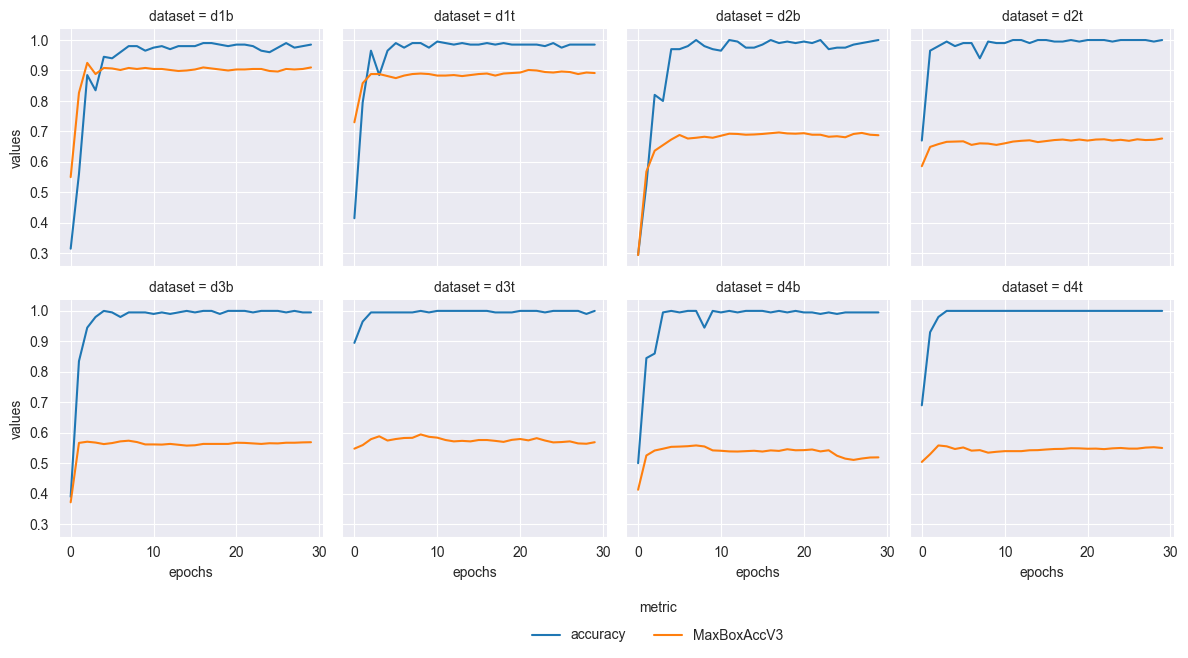
\includegraphics[width=\textwidth]{fig_loc_vs_acc_vgg16_gap_cam_synthetic.png}
    \caption[Classification versus CAM localization accuracy on VGG16-GAP for synthetic datasets]{Classification versus CAM localization accuracy on VGG16-GAP for synthetic datasets.}
    \caption*{Source: Author}
    \label{fig:loc_vs_acc_vgg16_gap_cam_synthetic}
    \end{center}
\end{figure}

Figure \ref{fig:loc_vs_acc_vgg16_gap_minmaxcam_synthetic} shows training classification and CAM MaxBoxAccV3 recall for model fine-tuned with MinMaxCAM regularization on the different datasets. Here, we observe that models trained for the t-variant datasets show a curve with decreasing MaxBoxAccV3 recall at later training epochs. This is in line with results in Table \ref{tab:maxboxaccv3_recall_vgg16_gap_synthetic}. As Wang \textit{et al.} \cite{wang2021minmaxcam} set out, the condition for common region regularization to work, is that a set of images for the same class should have different backgrounds. This clearly is not the case for the t-variant datasets.

\begin{figure}[ht]
    \begin{center}       
    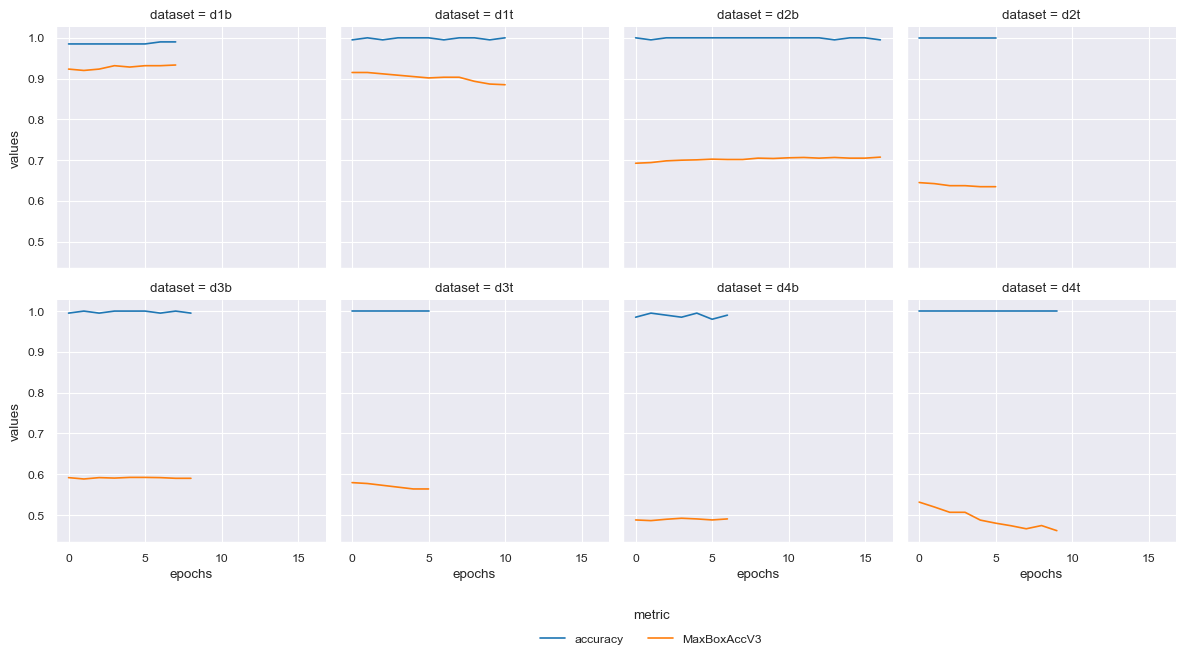
\includegraphics[width=\textwidth]{fig_loc_vs_acc_vgg16_gap_minmaxcam_synthetic.png}
    \caption[Classification versus MinMaxCAM localization accuracy on VGG16-GAP for synthetic datasets]{Classification versus MinMaxCAM localization accuracy on VGG16-GAP for synthetic datasets.}
    \caption*{Source: Author}
    \label{fig:loc_vs_acc_vgg16_gap_minmaxcam_synthetic}
    \end{center}
\end{figure}

\subsubsection{VGG16}
The localization results for VGG16 on the synthetic datasets are shown in Table \ref{tab:maxboxaccv3_recall_vgg16_base_synthetic} for MaxBoxAccV3 recall, in Table \ref{tab:maxboxaccv3_precision_vgg16_base_synthetic} for MaxBoxAccV3 precision, and in Table \ref{tab:pxap_vgg16_base_synthetic} for the PxAP metric. Note that CAM and MinMaxCAM methods cannot be used on VGG16 as this architecture has no \acrshort{gap} layer. Grad-CAM is used here as generalization of CAM.

\begin{table}[ht]
\centering
\begin{tabular}{lrrrrrrrr}
\toprule
 & \multicolumn{8}{c}{VGG16 synthetic (MaxBoxAccV3 recall)} \\
method & d1b & d1t & d2b & d2t & d3b & d3t & d4b & d4t \\
\cmidrule(lr){1-1} \cmidrule(lr){2-9} 
Grad-CAM & \color{teal} \bfseries 81.33 & 68.83 & 51.17 & 46.08 & 46.94 & 45.06 & 45.33 & 44.00 \\
Grad-CAM++ & \color{purple} \bfseries 72.17 & \color{purple} \bfseries 66.83 & \color{purple} \bfseries 37.58 & \color{purple} \bfseries 35.58 & \color{purple} \bfseries 36.33 & \color{purple} \bfseries 31.94 & \color{purple} \bfseries 35.29 & \color{purple} \bfseries 38.75 \\
Score-CAM & 77.50 & \color{teal} \bfseries 69.33 & \color{teal} \bfseries 55.33 & \color{teal} \bfseries 49.42 & \color{teal} \bfseries 50.50 & \color{teal} \bfseries 49.50 & \color{teal} \bfseries 48.08 & \color{teal} \bfseries 46.79 \\
\bottomrule
\end{tabular}
\caption[MaxBoxAccV3 recall for VGG16 on synthetic datasets]{MaxBoxAccV3 recall for VGG16 on synthetic datasets. Column-wise minimum and maximum are highlighted in red and green.}
\label{tab:maxboxaccv3_recall_vgg16_base_synthetic}
\end{table}

\begin{table}[ht]
\centering
\begin{tabular}{lrrrrrrrr}
\toprule
 & \multicolumn{8}{c}{VGG16 synthetic (MaxBoxAccV3 precision)} \\
method & d1b & d1t & d2b & d2t & d3b & d3t & d4b & d4t \\
\cmidrule(lr){1-1} \cmidrule(lr){2-9}
Grad-CAM & 53.29 & 43.62 & 53.78 & 46.13 & 47.38 & 44.70 & 47.99 & 48.13 \\
Grad-CAM++ & \color{purple} \bfseries 29.51 & \color{purple} \bfseries 29.45 & \color{purple} \bfseries 32.24 & \color{purple} \bfseries 29.36 & \color{purple} \bfseries 31.81 & \color{purple} \bfseries 25.84 & \color{purple} \bfseries 31.01 & \color{purple} \bfseries 35.49 \\
Score-CAM & \color{teal} \bfseries 54.05 & \color{teal} \bfseries 47.01 & \color{teal} \bfseries 58.24 & \color{teal} \bfseries 51.22 & \color{teal} \bfseries 52.48 & \color{teal} \bfseries 52.10 & \color{teal} \bfseries 52.36 & \color{teal} \bfseries 53.33 \\
\bottomrule
\end{tabular}
\caption[MaxBoxAccV3 precision for VGG16 on synthetic datasets]{MaxBoxAccV3 precision for VGG16 on synthetic datasets. Column-wise minimum and maximum are highlighted in red and green.}
\label{tab:maxboxaccv3_precision_vgg16_base_synthetic}
\end{table}

\begin{table}[ht]
\centering
\begin{tabular}{lrrrrrrrr}
\toprule
 & \multicolumn{8}{c}{VGG16 synthetic (PxAP)} \\
method & d1b & d1t & d2b & d2t & d3b & d3t & d4b & d4t \\
\cmidrule(lr){1-1} \cmidrule(lr){2-9}
Grad-CAM & \color{teal} \bfseries 69.83 & 59.06 & 57.35 & 45.12 & 51.73 & 52.00 & 56.18 & 54.84 \\
Grad-CAM++ & \color{purple} \bfseries 63.92 & \color{purple} \bfseries 58.11 & \color{purple} \bfseries 42.26 & \color{purple} \bfseries 34.54 & \color{purple} \bfseries 44.73 & \color{purple} \bfseries 38.77 & \color{purple} \bfseries 46.06 & \color{purple} \bfseries 47.34 \\
Score-CAM & 66.44 & \color{teal} \bfseries 60.73 & \color{teal} \bfseries 59.32 & \color{teal} \bfseries 52.59 & \color{teal} \bfseries 58.39 & \color{teal} \bfseries 59.53 & \color{teal} \bfseries 58.25 & \color{teal} \bfseries 58.74 \\
\bottomrule
\end{tabular}
\caption[PxAP for VGG16 on synthetic datasets]{PxAP for VGG16 on synthetic datasets. Column-wise minimum and maximum are highlighted in red and green.}
\label{tab:pxap_vgg16_base_synthetic}
\end{table}

A first observation is that the localization metrics for VGG16 are lower than those for the VGG16-GAP network. An intuitive explanation is that in the VGG16 network there is a less direct relationship between feature activation in the last convolutional layer and the predicted target due to the dense network between the convolutional backbone and the classification output. 

Another important observation is that Score-CAM is the best performing localization method, followed by Grad-CAM. and then by Grad-CAM++ by quite a large margin. The difference between Grad-CAM and Grad-CAM localization results for the VGG16 network seems counter-intuitive with findings of Chattopadhay \textit{et al.} \cite{chattopadhay2018grad}, that Grad-CAM++ is better at explaining multiple object instances than Grad-CAM. A possible indication could be that for the synthetic datasets, Grad-CAM++ seems to activate on larger areas, as illustrated in Fig. \ref{fig:vgg16_base_explanation}.

\begin{figure}[ht]
    \begin{center}
    \begin{subfigure}[b]{\textwidth}
         \centering
         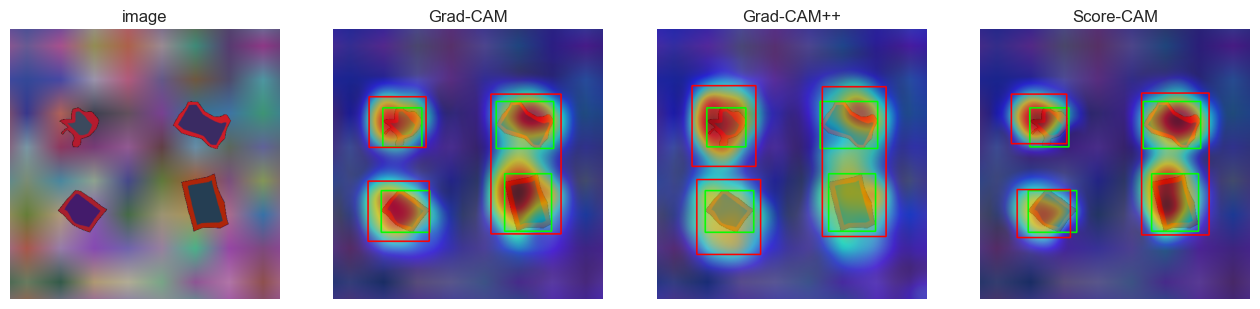
\includegraphics[width=\textwidth]{fig_vgg16_base_d4b.png}
         \caption{Explanation example from d4b dataset.}
         \label{fig:vgg16_base_explanation_d4b}
    \end{subfigure}
    \begin{subfigure}[b]{\textwidth}
         \centering
         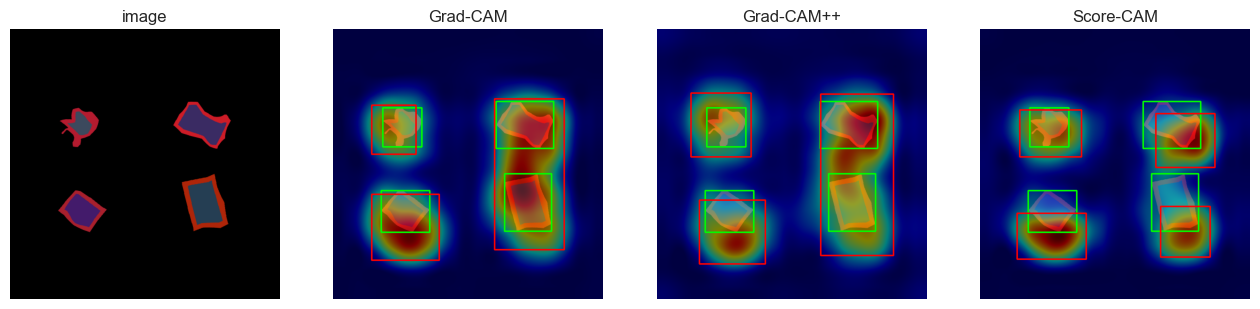
\includegraphics[width=\textwidth]{fig_vgg16_base_d4t.png}
         \caption{Explanation example from d4t dataset.}
         \label{fig:vgg16_base_explanation_d4t}
    \end{subfigure}
    \caption[Explanation maps for localization methods on VGG16 network]{Explanation maps for localization methods on VGG16 network. Heat maps show the activated image areas for the ground truth class. Annotations are given for ground truth (green) and predicted (red) bounding boxes.}
    \caption*{Source: Author}
    \label{fig:vgg16_base_explanation}
    \end{center}
\end{figure}

Finally, we see a similar trend in pair-wise discrepancies between b-variant and t-variant datasets having the same number of object instances as observed for the VGG16-GAP network.  

\subsubsection{ResNet-50}
Localization performance results for the ResNet-50 network on the synthetic dataset are illustrated in Table \ref{tab:maxboxaccv3_recall_resnet50_synthetic} for MaxBoxAccV3 recall, in Table \ref{tab:maxboxaccv3_precision_resnet50_synthetic} for MaxBoxAccV3 precision and in Table \ref{tab:pxap_resnet50_synthetic} for PxAP. Here Grad-CAM is not evaluated as it is identical to CAM for architectures with a \acrshort{gap} architecture.

\begin{table}[ht]
\centering
\begin{tabular}{lrrrrrrrr}
\toprule
 & \multicolumn{8}{c}{ResNet-50 synthetic (MaxBoxAccV3 recall)} \\
method & d1b & d1t & d2b & d2t & d3b & d3t & d4b & d4t \\
\cmidrule(lr){1-1} \cmidrule(lr){2-9}
CAM & \color{purple} \bfseries 84.00 & \color{purple} \bfseries 74.67 & \color{purple} \bfseries 67.08 & \color{purple} \bfseries 71.08 & \color{purple} \bfseries 62.89 & \color{purple} \bfseries 62.61 & \color{purple} \bfseries 59.29 & \color{purple} \bfseries 58.71 \\
Grad-CAM++ & 85.33 & 75.67 & \color{teal} \bfseries \underline{69.33} & 72.08 & \color{teal} \bfseries \underline{66.06} & 65.00 & \color{teal} \bfseries \underline{61.79} & \color{teal} \bfseries \underline{61.13} \\
Score-CAM & \color{teal} \bfseries \underline{85.50} & \color{teal} \bfseries \underline{77.00} & 68.92 & \color{teal} \bfseries 73.58 & 64.89 & \color{teal} \bfseries 65.50 & 61.63 & 60.58 \\
\cmidrule(lr){1-1} \cmidrule(lr){2-9}
MinMaxCAM & 80.33 & \color{purple} \bfseries \underline{68.17} & \color{purple} \bfseries \underline{59.17} & \color{purple} \bfseries \underline{59.08} & \color{purple} \bfseries \underline{56.50} & \color{purple} \bfseries \underline{56.11} & \color{purple} \bfseries \underline{55.92} & \color{purple} \bfseries \underline{52.87} \\
Grad-CAM++ & \color{teal} \bfseries 80.83 & 69.17 & \color{teal} \bfseries 63.83 & 61.92 & \color{teal} \bfseries 61.00 & \color{teal} \bfseries 59.94 & \color{teal} \bfseries 58.96 & \color{teal} \bfseries 57.08 \\
Score-CAM & \color{purple} \bfseries \underline{79.00} & \color{teal} \bfseries 71.17 & 61.00 & \color{teal} \bfseries 62.50 & 58.44 & 59.11 & 58.71 & 56.83 \\
\bottomrule
\end{tabular}
\caption[MaxBoxAccV3 recall for ResNet-50 on synthetic datasets]{MaxBoxAccV3 recall for ResNet-50 on synthetic datasets. First 3 rows are results for model trained without regularization. Last 3 rows show results for model trained with MinMaxCAM regularization. Column-wise minimum and maximum per sub-table are highlighted in red and green. Global column-wise minimum and maximum are underlined.}
\label{tab:maxboxaccv3_recall_resnet50_synthetic}
\end{table}

\begin{table}[ht]
\centering
\begin{tabular}{lrrrrrrrr}
\toprule
 & \multicolumn{8}{c}{ResNet-50 synthetic (MaxBoxAccV3 precision)} \\
method & d1b & d1t & d2b & d2t & d3b & d3t & d4b & d4t \\
\cmidrule(lr){1-1} \cmidrule(lr){2-9}
CAM & \color{purple} \bfseries 75.30 & \color{purple} \bfseries 59.95 & \color{purple} \bfseries 69.48 & \color{purple} \bfseries 73.63 & \color{purple} \bfseries 68.29 & \color{purple} \bfseries 66.17 & \color{purple} \bfseries 65.83 & \color{purple} \bfseries 65.50 \\
Grad-CAM++ & 76.75 & 61.45 & \color{teal} \bfseries \underline{70.99} & 73.84 & \color{teal} \bfseries \underline{70.14} & 67.96 & 66.94 & \color{teal} \bfseries \underline{66.57} \\
Score-CAM & \color{teal} \bfseries \underline{77.58} & \color{teal} \bfseries \underline{64.77} & 69.51 & \color{teal} \bfseries \underline{74.60} & 69.25 & \color{teal} \bfseries \underline{68.70} & \color{teal} \bfseries \underline{67.75} & 65.82 \\
\cmidrule(lr){1-1} \cmidrule(lr){2-9}
MinMaxCAM & 70.21 & \color{purple} \bfseries \underline{49.82} & \color{purple} \bfseries \underline{61.23} & \color{purple} \bfseries \underline{60.03} & \color{purple} \bfseries \underline{61.27} & \color{purple} \bfseries \underline{59.88} & \color{purple} \bfseries \underline{62.59} & \color{purple} \bfseries \underline{58.82} \\
Grad-CAM++ & \color{teal} \bfseries 71.31 & 53.73 & \color{teal} \bfseries 64.93 & \color{teal} \bfseries 62.81 & \color{teal} \bfseries 63.74 & \color{teal} \bfseries 62.68 & \color{teal} \bfseries 63.85 & \color{teal} \bfseries 61.90 \\
Score-CAM & \color{purple} \bfseries \underline{68.87} & \color{teal} \bfseries 55.41 & 61.61 & 62.07 & 62.13 & 62.09 & 63.64 & 61.30 \\
\bottomrule
\end{tabular}
\caption[MaxBoxAccV3 precision for ResNet-50 on synthetic datasets]{MaxBoxAccV3 precision for ResNet-50 on synthetic datasets. First 3 rows are results for model trained without regularization. Last 3 rows show results for model trained with MinMaxCAM regularization. Column-wise minimum and maximum per sub-table are highlighted in red and green. Global column-wise minimum and maximum are underlined.}
\label{tab:maxboxaccv3_precision_resnet50_synthetic}
\end{table}

\begin{table}[ht]
\centering
\begin{tabular}{lrrrrrrrr}
\toprule
 & \multicolumn{8}{c}{ResNet-50 synthetic (PxAP)} \\
method & d1b & d1t & d2b & d2t & d3b & d3t & d4b & d4t \\
\cmidrule(lr){1-1} \cmidrule(lr){2-9} 
CAM & \color{purple} \bfseries 76.85 & \color{purple} \bfseries 65.98 & \color{purple} \bfseries 75.60 & \color{purple} \bfseries 77.27 & 75.32 & \color{purple} \bfseries 73.97 & 74.00 & \color{purple} \bfseries 71.46 \\
Grad-CAM++ & \color{teal} \bfseries 78.02 & 68.86 & \color{teal} \bfseries 76.97 & 78.03 & \color{teal} \bfseries 76.93 & 74.69 & \color{teal} \bfseries 75.31 & 72.10 \\
Score-CAM & 77.97 & \color{teal} \bfseries 69.36 & 76.09 & \color{teal} \bfseries 79.37 & \color{purple} \bfseries 74.63 & \color{teal} \bfseries 75.58 & \color{purple} \bfseries 72.83 & \color{teal} \bfseries 72.92 \\
\cmidrule(lr){1-1} \cmidrule(lr){2-9} 
MinMaxCAM & \color{purple} \bfseries 71.11 & \color{purple} \bfseries 56.26 & \color{purple} \bfseries 63.38 & \color{purple} \bfseries 66.11 & 67.64 & \color{purple} \bfseries 66.99 & \color{purple} \bfseries 68.71 & \color{purple} \bfseries 64.74 \\
Grad-CAM++ & \color{teal} \bfseries 72.56 & 59.92 & \color{teal} \bfseries 66.74 & 68.09 & \color{teal} \bfseries 70.15 & \color{teal} \bfseries 69.25 & \color{teal} \bfseries 70.83 & 66.89 \\
Score-CAM & 71.43 & \color{teal} \bfseries 61.04 & 65.57 & \color{teal} \bfseries 68.20 & \color{purple} \bfseries 67.23 & 68.20 & 69.15 & \color{teal} \bfseries 67.20 \\
\bottomrule
\end{tabular}
\caption[PxAP for ResNet-50 on synthetic datasets]{PxAP for ResNet-50 on synthetic datasets. First 3 rows are results for model trained without regularization. Last 3 rows show results for model trained with MinMaxCAM regularization. Column-wise minimum and maximum per sub-table are highlighted in red and green. Global column-wise minimum and maximum are underlined.}
\label{tab:pxap_resnet50_synthetic}
\end{table}

A similar trend as for VGG16-GAP and VGG16 networks can be observed: Localization performance decreases for increasing number of object instances in images. 

Grad-CAM++ and Score-CAM localization methods perform better than CAM, both for the non-regularized model and for the MinMaxCAM-regularized model. Chattopadhay \textit{et al.} \cite{chattopadhyay2017grad} visually illustrated how taking a weighted combination of positive partial derivatives instead of a global average solves the problem of identifying multiple occurrences of the same class in an image and improper object localization. We quantitatively show that this statement holds for most synthetic datasets on the ResNet-50 network.

The MinMaxCAM-regularized model has lower localization performance than the non-regularized one for the ResNet-50 network. There is room for improvement as we haven't optimized the hyper parameters for MinMaxCAM. Still, it can be observed that both Grad-CAM++ and Score-CAM both improve on the CAM localization results.

\subsection{ImageNet dataset}
In this section we evaluate the localization methods on the ImageNet validation dataset. Multi-instance localization metrics MaxBoxAccV3 recall and precision are used as in previous sections. In addition we report the MaxBoxAcc and MaxBoxAccV2 metrics to benchmark our trained models with results provided by Choe \textit{et al.} \cite{choe2020evaluating} where appropriate. \acrfull{pxap} cannot be used as localization metric as the ImageNet dataset has no ground truth segmentation masks. In following sections, results for VGG16-GAP and ResNet-50 architectures are discussed.

\subsubsection{VGG16-GAP}
We modified a pre-trained VGG16 network into the VGG16-GAP network by replacing the dense network of VGG16 with a \acrshort{gap} layer followed by a single fully connected layer. This newly constructed network is fine-tuned until the loss of the validation dataset hasn't decreased for five consecutive training epochs. The localization results of VGG16-GAP on the ImageNet validation dataset are illustrated in Table \ref{tab:metrics_vgg16_gap_imagenet}.

\begin{table}[ht]
\centering
\begin{tabular}{lrrrr}
\toprule
 & & & \multicolumn{2}{c}{MaxBoxAccV3} \\
method & MaxBoxAcc & MaxBoxAccV2 & precision & recall \\
\cmidrule(lr){1-1} \cmidrule(lr){2-5}
CAM & 61.19 & 60.22 & \color{purple} \bfseries 36.73 & 38.44 \\
Grad-CAM++ & \color{teal} \bfseries 61.29 & \color{teal} \bfseries 60.43 & 36.87 & \color{teal} \bfseries 38.66 \\
Score-CAM & \color{purple} \bfseries 58.44 & \color{purple} \bfseries 57.56 & \color{teal} \bfseries 37.33 & \color{purple} \bfseries 36.48 \\
\bottomrule
\end{tabular}
\caption[Localization metrics for VGG16-GAP on ImageNet]{Localization metrics for VGG16-GAP on ImageNet. Column-wise minimum and maximum are highlighted in red and green.}
\label{tab:metrics_vgg16_gap_imagenet}
\end{table}

The values for the metrics MaxBoxAcc ($61.19$) and MaxBoxAccV2 ($60.22$) for the \acrshort{cam} method closely match the results reported by Choe \textit{et al.} \cite{choe2020evaluating}. Our VGG16-GAP model is thus able to reproduce the results in the \acrshort{wsol} evaluation paper.

The MaxBoxAccV3 precision and recall values for VGG16-GAP on the ImageNet dataset are much lower than the values for the synthetic dataset. This is to be expected as the ImageNet dataset is far more complex: It has 1000 different classes and a training dataset of 1.2 million images, where the synthetic datasets have only 9 different classes with a training dataset of 1000 images. The model trained on the ImageNet dataset has a classification accuracy of 67.1\%, where classification accuracy for models trained on the synthetic datasets is close to 100\%. 

MaxBoxAccV3 recall for Score-CAM is about 2 percentage points lower than CAM and Grad-CAM++. An intuitive explanation for the lower Score-CAM score could be that Score-CAM tends to generate more focused score maps than Grad-CAM++, resulting in less accurate bounding box estimations. 

The multi-instance localization metrics are expected to be determined predominantly by single-instance images in the ImageNet dataset as they are the majority of images in the validation dataset (Fig. \ref{fig:imagenet_instance_distribution}. It would be interesting to split up the ImageNet training and validation datasets along the number of object instances in images to evaluate localization performance in function of the number of object instances. We see this as future work.

Due to time constraints, we haven't trained a MinMaxCAM-regularized model for the VGG16-GAP network on ImageNet.

\subsubsection{ResNet-50}

For the ResNet-50 network we evaluate CAM, Grad-CAM++ and Score-CAM on the ImageNet validation dataset, both for a model trained without regularization, and on a model trained with MinMaxCAM regularization. The results of these experiments are illustrated in Table \ref{tab:metrics_resnet50_imagenet}, where the method denoted as MinMaxCAM shows the results for the MinMaxCAM-regularized model evaluated with the CAM method. 

The MaxBoxAcc and MaxBoxAccV2 metrics for the CAM method evaluated on the unregularized model have lower values than those reported by Choe \textit{et al.} \cite{choe2020evaluating} (57.60 and 57.25 versus 64.2 and 63.7). An explanation for this discrepancy, most likely is that we used a pre-trained ResNet-50 model where the authors of the mentioned paper did a grid search on hyper parameters to improve localization. 

The MaxBoxAccV3 metric has slightly lower values than the ones we reported for the VGG16-GAP network, but the same trend can be observed: The highest recall is obtained by the Grad-CAM++ method and the Score-CAM recall is about two percentage points below Grad-CAM++'s value. 

Where MaxBoxAccV3 recall differences between non-regularized and regularized models are marginal, MaxBoxAccV3 precision has improved substantially for the localization methods evaluated on the regularized model when compared with the non-regularized model. indicating that localization methods using this model produce fewer false positives.

MaxBoxAcc and MaxBoxAccV2 values are slightly higher for the MinMaxCAM-regularized model than for the non-regularized model. This is in contrast with the results noted by Wang \textit{et al.} \cite{wang2021minmaxcam}, who illustrated that MinMaxCAM improves MaxBoxAcc by 2.5 percentage points compared to CAM. We haven't reproduced the results of the authors of the MinMaxCAM paper \cite{wang2021minmaxcam}, due to lack of reference values for the regularization weights.

\begin{table}[ht]
\centering
\begin{tabular}{lrrrr}
\toprule
 & & & \multicolumn{2}{c}{MaxBoxAccV3} \\
method & MaxBoxAcc & MaxBoxAccV2 & precision & recall \\
\cmidrule(lr){1-1} \cmidrule(lr){2-5}
CAM & 57.60 & 57.25 & 30.55 & 36.58 \\
Grad-CAM++ & \color{teal} \bfseries 59.40 & \color{teal} \bfseries 58.55 & \color{teal} \bfseries 31.17 & \color{teal} \bfseries \underline{37.53} \\
Score-CAM & \color{purple} \bfseries \underline{56.19} & \color{purple} \bfseries \underline{56.35} & \color{purple} \bfseries \underline{29.60} & \color{purple} \bfseries \underline{35.92} \\
\cmidrule(lr){1-1} \cmidrule(lr){2-5}
MinMaxCAM & \color{purple} \bfseries 58.81 & \color{purple} \bfseries 57.26 & \color{teal} \bfseries \underline{43.70} & \color{purple} \bfseries 36.02 \\
Grad-CAM++ & \color{teal} \bfseries \underline{60.87} & \color{teal} \bfseries \underline{58.92} & 41.81 & \color{teal} \bfseries 37.12 \\
Score-CAM & 60.00 & 58.10 & \color{purple} \bfseries 38.70 & 36.53 \\
\bottomrule
\end{tabular}
\caption[Localization metrics for ResNet-50 on ImageNet]{Localization metrics for ResNet-50 on ImageNet. First 3 rows are results for model trained without regularization. Last 3 rows show results for model trained with MinMaxCAM regularization. Column-wise minimum and maximum per sub-table are highlighted in red and green. Global column-wise minimum and maximum are underlined.}
\label{tab:metrics_resnet50_imagenet}
\end{table}

In chapter \ref{ch:methodology} we reported the distribution of object instances over the images in the ImageNet validation dataset (Fig. \ref{fig:imagenet_instance_distribution}. Because the vast majority of images in the dataset has only one object instance, the localization results may be biased towards those images. Therefore, we have split the ImageNet validation dataset into different datasets, so that each dataset has only images with fixed number of object instances. We then evaluated the CAM localization method separately on each of these datasets.

The MaxBoxAccV3 recall results for these experiments are shown in Fig. \ref{fig:resnet50_imagenet_inst_recall}. We observe that recall performance depends on the number of object instances in the images. Recall is highest for the single-instance dataset, and significantly drops significantly as more object instances are in the images of a dataset. For ImageNet datasets with eight or more instance, recall seems to be rather similar. We observed a similar pattern for the synthetic datasets: Lower recall for those datasets having more object instances in images.

The ImageNet dataset with single-instance images has a MaxBoxAccV3 recall of 63.38, which is close to the MaxBoxAccV2 value of 57.25 in Table \ref{tab:metrics_resnet50_imagenet}. It can be shown that for single-instance datasets, MaxBoxAccV2 and MaxBoxAccV3 are identical, as in this case, the number of images equals the number ground-truth bounding boxes, and from equations \ref{eq:boxacc}, \ref{eq:maxboxaccv2}, \ref{eq:boxaccv2} and \ref{eq:maxboxaccv3}, we can derive that MaxBoxAccV2 equals MaxBoxAccV3. The difference in the results is because the MaxBoxAccV2 value from Table \ref{tab:metrics_resnet50_imagenet} was measured on the complete ImageNet validation dataset, including images with more than one object instance.
\begin{figure}[ht]
    \begin{center}       
    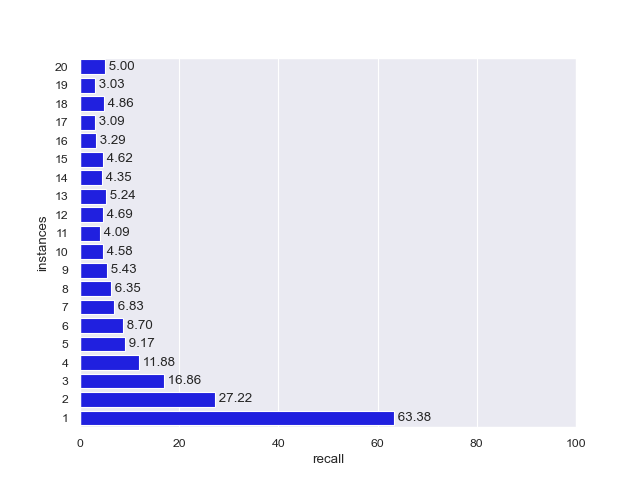
\includegraphics[width=0.8\textwidth]{fig_resnet50_imagenet_inst_recall.png}
    \caption[CAM MaxBoxAccV3 recall on ResNet-50 for ImageNet split across number object instances]{CAM MaxBoxAccV3 recall on ResNet-50 for ImageNet split across number object instances.}
    \caption*{Source: Author}
    \label{fig:resnet50_imagenet_inst_recall}
    \end{center}
\end{figure}

Fig. \ref{fig:resnet50_imagenet_inst_precision} illustrated MaxBoxAccV3 precision for the ImageNet datasets split by number of object instances. For  the first four datasets (instances 1 till 4), we see a drop in precision as more instances are present in images. When dataset images have more object instances, precision values don't seem to correlate with the number of instances. That means that the localization method is not generating relatively more false positives are more object instances are present in the images.

\begin{figure}[ht]
    \begin{center}       
    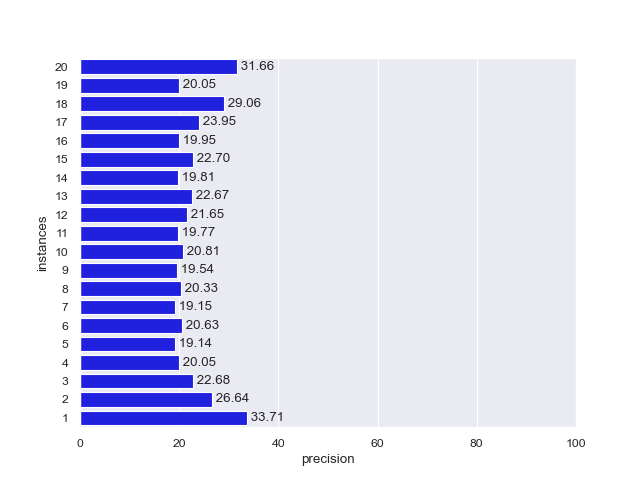
\includegraphics[width=0.8\textwidth]{fig_resnet50_imagenet_inst_precision.png}
    \caption[CAM MaxBoxAccV3 precision on ResNet-50 for ImageNet split across number object instances]{CAM MaxBoxAccV3 precision on ResNet-50 for ImageNet split across number object instances.}
    \caption*{Source: Author}
    \label{fig:resnet50_imagenet_inst_precision}
    \end{center}
\end{figure}

Intuitively, the more object instances in an image, the closer they are, and the higher the probability that the localization method will localize groups of instances as a single instance. Missing object instance locations will have more impact on recall than on precision.
 
\section{Computational complexity}
In this section we evaluate the computational complexity of localization methods CAM, Grad-CAM++ and Score-CAM. MinMaxCAM and Grad-CAM are not measured as MinMaxCAM uses the same localization method as CAM and Grad-CAM has the same order of complexity as Grad-CAM++ due to the equal number of forward and backward passes (see Table \ref{tab:complexity_theoretical}). We measure the localization method runtime for ResNet-50 network on the 50000 images of the ImageNet validation dataset. 

The runtime of the localization methods is measured as the time it takes to compute the score map of the images. For efficiency reasons, we process batches of images for score map computation, thus the runtime measurements are also performed on batches of images. Mean and standard deviation are then computed over all batches of the dataset, and total runtime is the sum of the runtime of all batches. Runtime computation excludes operations to load and preprocess the images. 

The results for each method are illustrated in Table \ref{tab:runtime_resnet50_imagenet}. The batch size is listed per method as it should be taken into consideration when interpreting the mean and standard deviation values.

\begin{table}[ht]
\centering
\begin{tabular}{lrrrr}
\toprule
\multicolumn{2}{c}{} & \multicolumn{3}{c}{runtime (ms)} \\
method & batch size (images) & sum & mean & std \\
\cmidrule(lr){1-2} \cmidrule(lr){3-5}
CAM & 512 & 309209 & 3155 & 225 \\
Grad-CAM++ & 128 & 804349 & 2057 & 140 \\
MinMaxCAM & 512 & 299392 & 3055 & 982 \\
Score-CAM & 512 & \color{teal} \bfseries 97763413 & \color{teal} \bfseries 997585 & \color{teal} \bfseries 34463\\
\bottomrule
\end{tabular}
\caption[Method runtime for ResNet-50 on ImageNet validation dataset]{Method runtime for ResNet-50 on ImageNet validation dataset.  Column-wise maximum is highlighted in bold green.}
\label{tab:runtime_resnet50_imagenet}
\end{table}

We observe that Grad-CAM++ takes nearly three times the runtime of the CAM method. The major difference is that Grad-CAM++ requires a backward pass after each forward pass to compute gradients. This indicates that backward passes are more costly than forward passes.

Each method computes a score map as a weighted combination of feature maps in the final convolutional layer. CAM computes as weights the parameters learned in the single fully connected layer, which is a very cheap operation. Grad-CAM and Grad-CAM++ compute weights from feature activations and the back-propagated gradients in the final convolutional layer.

The most computationally costly method by far is Score-CAM. This method computes the weights for the feature maps by feeding the network with the product of each feature map with the original image to obtain the classification score after softmax. The classification scores are then used as weights. As ResNet-50 has 2048 channels in its final convolutional layer, this is an expensive operation.

\section{Localization improvements} \label{sec:exp_loc_improvements}

Using the iterative localization method proposed in section \ref{sec:method_localization_improvement}, we analyze the effect of this method for VGG16-GAP and ResNet-50 architectures on the synthetic and ImageNet datasets. We use the same models that were trained for the non-iterative approach.

\subsection{Recall versus precision}
The aim of the iterative approach is to improve the accurate localization of ground truth object instances. This localization accuracy is measured by the MaxBoxAccV3 metric, i.e. the recall. If we would have a localization method that exhaustively generates bounding boxes of different granularity, then such method would accurately localize most object instances and thus have a high recall value. At the same time this method would suffer from a lot of false positives, i.e., many of the predicted object localization instances would not match with the actual ground localization annotations. Hence, precision would be very low. To measure the impact of the iterative localization method we want to measure both precision and recall. Ideally, we would like to have a localization method that has good precision and recall.

\subsection{Evaluation approach}
In our iterative localization approach, we apply different mask strategies, bounding box merge strategies and iteration stop criteria in our experiments. The different parameters and their possible values are illustrated in Table \ref{tab:iterative_localizaton_parameters}. Due to the number of possible parameter combinations, we have to compare a lot of results. It is not feasible to represent these results in a single table and draw conclusions from it.

\begin{table}[ht]
\centering
\begin{tabular}{ll}
\toprule
Parameter & Values\\
\cmidrule(lr){1-2}
Localization method & CAM, Grad-CAM++, Score-CAM, MinMaxCAM \\
Mask strategy & zero, mean, random \\
Merge strategy & add, drop, unify \\
Classification score drop threshold & 0.25, 0.5, 1.0 \\
\bottomrule
\end{tabular}
\caption[Parameters for the iterative localization approach]{Parameters for the iterative localization approach.}
\label{tab:iterative_localizaton_parameters}
\end{table}

Therefore we graphically represent and interpret the results as follows:
\begin{itemize}
    \item Per dataset, network and localization method, we create a two-dimensional plot with recall on the horizontal axis and precision on the vertical axis. In this plot, for each of the different combinations of mask strategies, merge strategies and stop criteria, an experiment is run and its resulting precision and recall are added to the plot.
    \item The precision and recall for the non-iterative approach is plotted as two orthogonal lines: A horizontal line for precision and vertical line for recall. We use the precision and recall from the non-iterative approach as baseline to compare with results from the iterative approach.
    \item The horizontal and vertical lines of the baseline create four quadrants which allow easy graphical interpretation of iterative localization results depending in which quadrant a result is situated.
    \begin{itemize}
        \item Bottom left: Precision and recall are worse than the baseline.
        \item Top left: Precision is better and recall is worse than baseline.
        \item Bottom right: Recall is better and precision is worse than baseline.
        \item Top right: Precision and recall are better than the baseline.
    \end{itemize}
\end{itemize}

\subsection{Evaluation for VGG16-GAP on synthetic datasets}
Here we evaluate the results of the iterative localization for the VGG16-GAP network on the synthetic test datasets. We only evaluate datasets that have images with a background to analyse the effect of using different bounding box mask strategies. The localization methods used are CAM, Grad-CAM++, Score-CAM and MinMaxCAM. The former three methods are evaluated on a model trained without regularization while the latter is evaluated on a model trained with MinMaxCAM regularization.

The MaxBoxAccV3 precision and recall of the iterative localization experiments for the different localization methods, mask strategies, merge strategies and iteration stop criteria on the synthetic dataset d1b, are illustrated in Fig. \ref{fig:prec_iter_vgg16_gap_syn_d1b}.

\begin{figure}[ht]
    \begin{center}       
    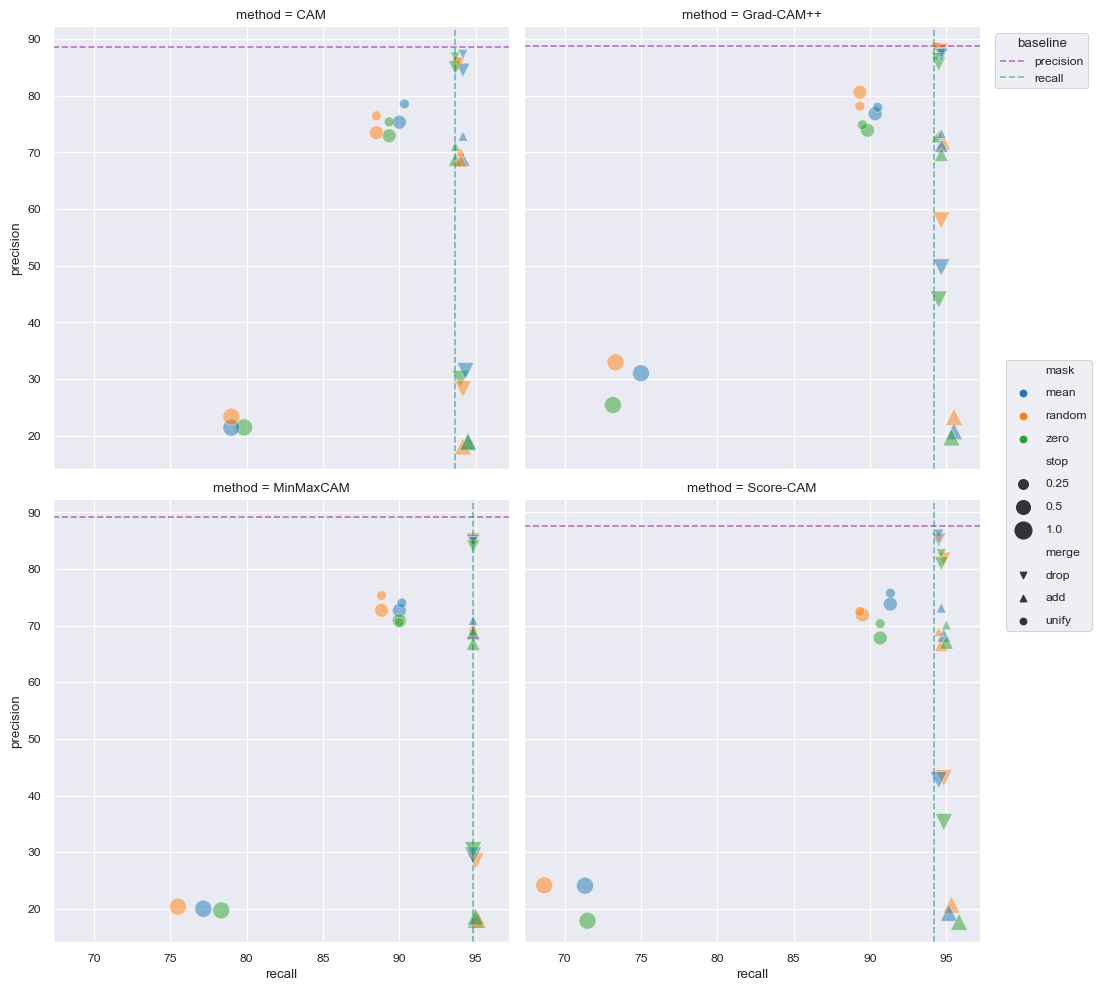
\includegraphics[width=1.0\textwidth]{images/fig_iter_vgg16_gap_syn_d1b.png}
    \caption[Iterative localization performance for VGG16-GAP on synthetic dataset d1b]{Iterative localization performance for VGG16-GAP on synthetic dataset d1b. The cross-hair lines mark the best precision and recall for non-iterative localization.}
    \caption*{Source: Author}
    \label{fig:prec_iter_vgg16_gap_syn_d1b}
    \end{center}
\end{figure}

When comparing with the baseline, we observe that for all methods except MinMaxCAM, both precision and recall can be improved by using the 'drop' merge strategy, when the classification score drop threshold 0.25 is used. As threshold 1.0 actually means that there is no stop criterion, it's easy to see that this threshold has the worst precision for any mask or merge strategy. The 'add' merge strategy improves recall but at a decreased precision cost, as this strategy will create more false positives. The relatively small gain in recall is to be expected for a dataset with single-instance object images where the baseline already has a high localization performance.

Iterative localization results for the d2b dataset are shown in Fig. \ref{fig:prec_iter_vgg16_gap_syn_d2b}. Looking at the upper right quadrant, we can observe that there are iterative localization methods that improve both precision and recall. The iterative methods applying the mean mask strategy, unify merge strategy and a stop criterion with classification drop threshold of 0.25 or 0.5 provide the best precision and recall improvements compared to the baseline.

The 'add' merge strategy combined with iteration drop criterion 1.0 gives the highest recall improvement but at the cost of severe precision drop. The worst performing approach is the 'unify' merge strategy with drop criterion 1.0. Intuitively, masking images with bounding boxes found in previous iterations, and unifying newly predicted bounding boxes with overlapping boxes of previous iterations, increases the risk of no longer matching predicted bounding boxes with ground truth boxes, and thus impacting recall.

\begin{figure}[ht]
    \begin{center}       
    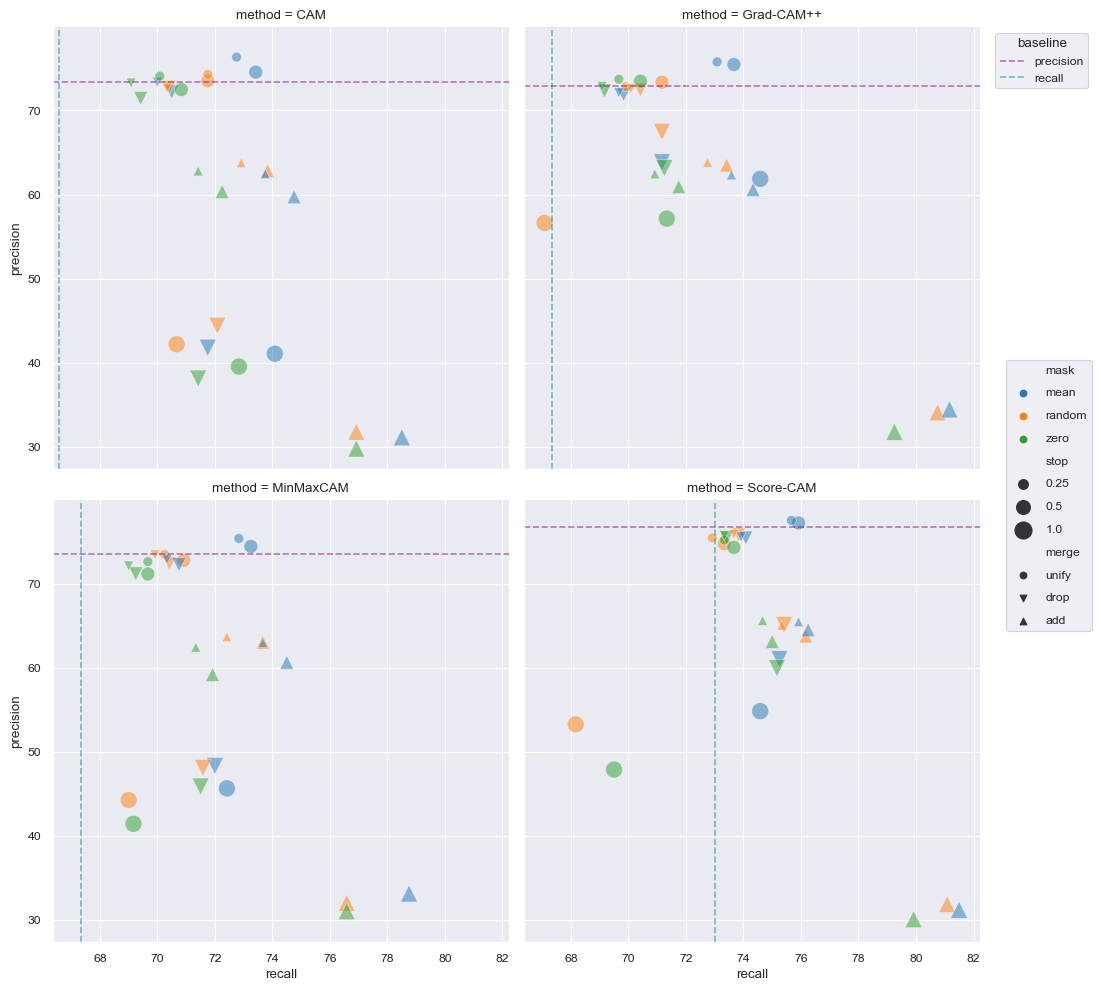
\includegraphics[width=1.0\textwidth]{images/fig_iter_vgg16_gap_syn_d2b.png}
    \caption[Iterative localization performance for VGG16-GAP on synthetic dataset d2b]{Iterative localization performance for VGG16-GAP on synthetic dataset d2b. The cross-hair lines mark the best precision and recall for non-iterative localization.}
    \caption*{Source: Author}
    \label{fig:prec_iter_vgg16_gap_syn_d2b}
    \end{center}
\end{figure}

Fig. \ref{fig:prec_iter_vgg16_gap_syn_d3b} illustrates the iterative localization results for the d3b dataset. We see that the iterative approach can improve both precision and recall for all localization methods. Applying the 'mean' mask strategy, 'unify' merge strategy and stop criterion threshold of 0.25 or 0.5 seems to be the best combination. This combination also improved both recall and precision for the d2b dataset.

\begin{figure}[ht]
    \begin{center}       
    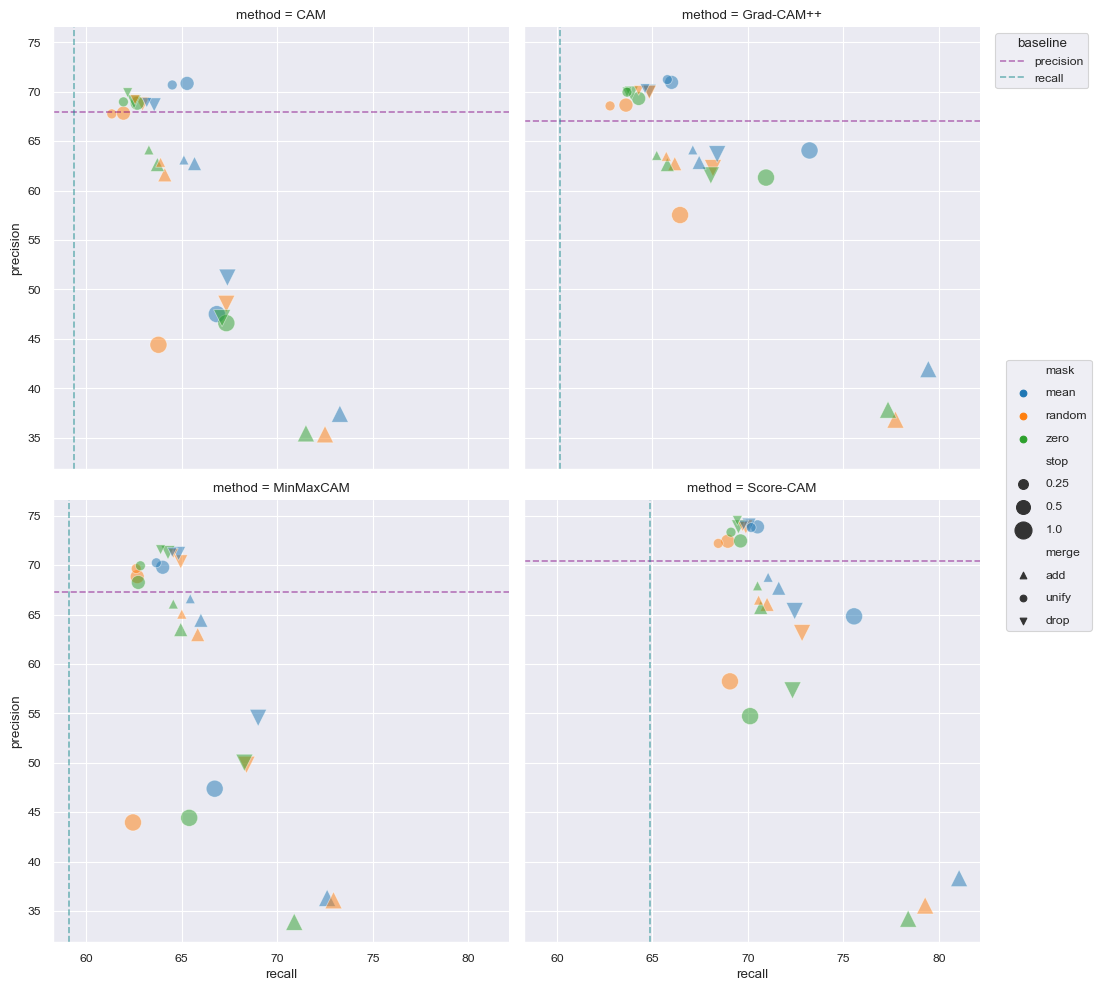
\includegraphics[width=1.0\textwidth]{images/fig_iter_vgg16_gap_syn_d3b.png}
    \caption[Iterative localization performance for VGG16-GAP on synthetic dataset d3b]{Iterative localization performance for VGG16-GAP on synthetic dataset d3b. The cross-hair lines mark the best precision and recall for non-iterative localization.}
    \caption*{Source: Author}
    \label{fig:prec_iter_vgg16_gap_syn_d3b}
    \end{center}
\end{figure}

The iterative localization metrics for the d4b dataset are shown in Fig. \ref{fig:prec_iter_vgg16_gap_syn_d4b}. Both precision and recall can be improved for all methods but MinMaxCAM, by applying the drop or unify merge strategy combined with zero mask strategy and a classification score drop threshold of 0.25. The 'add' merge strategy with stop threshold 1.0 provides the highest gain in recall at the cost of substantially decreasing precision.

\begin{figure}[ht]
    \begin{center}       
    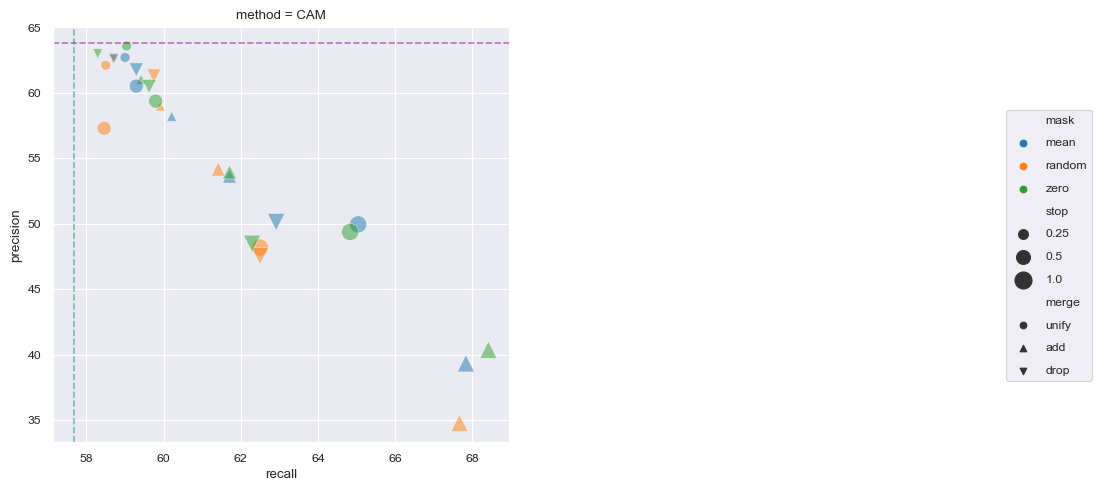
\includegraphics[width=1.0\textwidth]{images/fig_iter_vgg16_gap_syn_d4b.png}
    \caption[Iterative localization performance for VGG16-GAP on synthetic dataset d4b]{Iterative localization performance for VGG16-GAP on synthetic dataset d4b. The cross-hair lines mark the best precision and recall for non-iterative localization.}
    \caption*{Source: Author}
    \label{fig:prec_iter_vgg16_gap_syn_d4b}
    \end{center}
\end{figure}

\subsection{Evaluation for ResNet-50 on ImageNet dataset}

The results of the iterative localization methods for the ResNet-50 network, evaluated on the ImageNet validation dataset, are shown in Fig. \ref{fig:prec_iter_resnet50_imagenet}. The best performing methods are those that are positioned closest to the upper right corner of the plot. Observing the plots for all localization methods, we can see two distinct groups: One group that improves recall at the cost of decreasing precision, and another group that performs worse for both precision and recall when compared to the baseline.

The first group consists of the methods that apply as merge strategy either 'drop' or 'add', where the 'add' strategy gives a substantially higher gain in recall, but at a higher drop in precision. In this group, there is an almost linear relationship between precision and recall and the applied classification score drop threshold for a certain merge strategy. In the second group are the iterative localization methods that apply a unify merge strategy. Intuitively, unifying predicted bounding boxes from previous iterations with newly predicted bounding boxes increases the risk generating larger but few bounding boxes, and thus impacting both precision and recall.

\begin{figure}[ht]
    \begin{center}       
    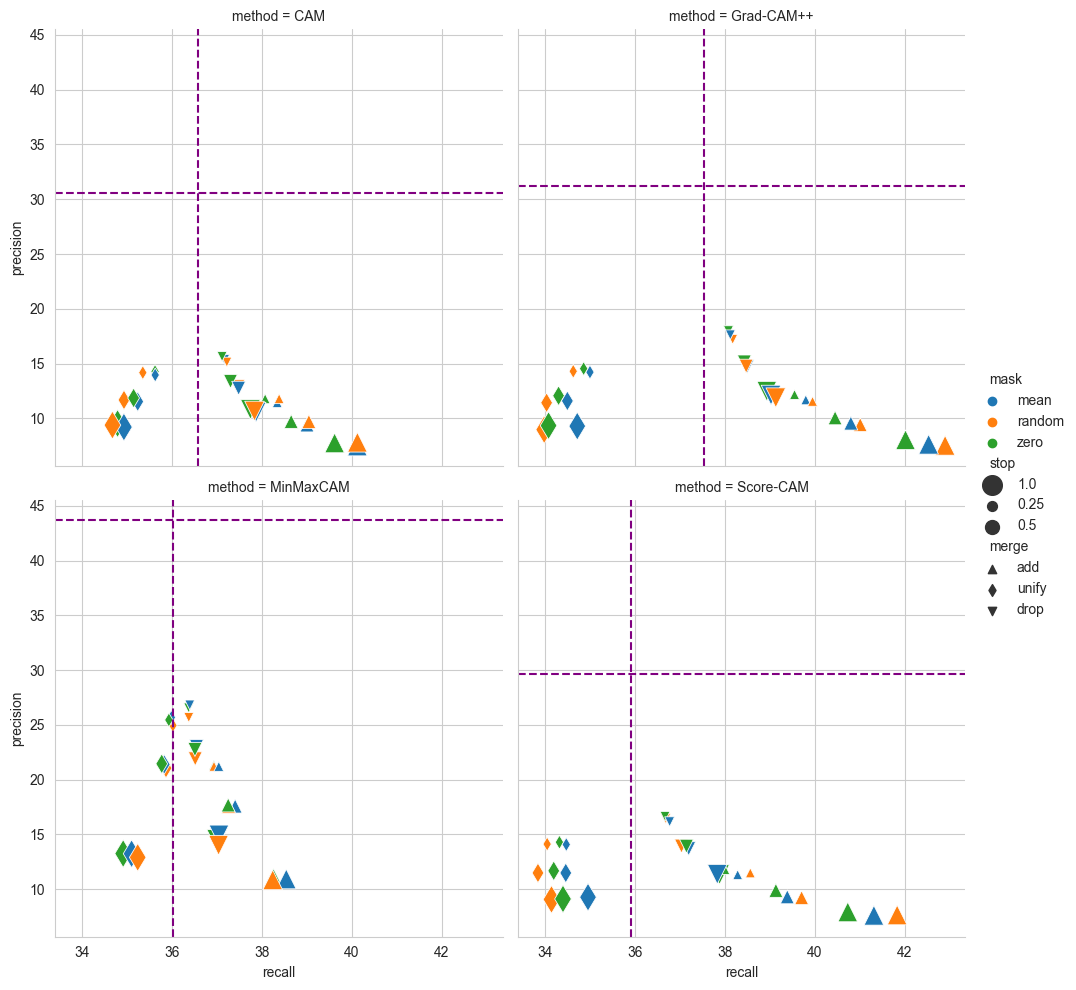
\includegraphics[width=1.0\textwidth]{fig_iter_resnet50_imagenet.png}
    \caption[Iterative localization performance for ResNet-50 on ImageNet dataset]{Iterative localization performance for ResNet-50 on ImageNet dataset. The cross-hair lines mark the best precision and recall for non-iterative localization.}
    \caption*{Source: Author}
    \label{fig:prec_iter_resnet50_imagenet}
    \end{center}
\end{figure}


\chapter{Discussion} \label{ch:discussion}

\section{Trends in experiments}
In general we found that for the synthetic datasets with multiple object instances, the best localization results are obtained by the Score-CAM for VGG16-GAP and VGG16 and by Grad-CAM++ for ResNet-50. Grad-CAM++ also performs best for the ImageNet dataset, both on VGG16-GAP and on ResNet-50. These quantitative evaluations confirm the promising results for multi-instance visualization observed by Wang \textit{et al.} \cite{wang2020score} and Chattopadhay \textit{et al.} \cite{chattopadhay2018grad}.

Score-CAM is not performing as good as the other localization methods for the ImageNet datasets, both on VGG16-GAP and on ResNet-50. As the majority of images in the ImageNet dataset has only one object instance of the target class, the promising results for multi-instance detection by Score-CAM do not weigh in the localization results for ImageNet. The fact that Score-CAM computes its score maps based on the score of the target class (Wang \textit{et al. \cite{wang2020score}} and because the classification accuracy for the ImageNet dataset is much lower than for the synthetic datasets, may further explain why Score-CAM is not performing as well for ImageNet as for the synthetic datasets.


In the iterative localization experiments, we found that the Grad-CAM++ and Score-CAM localization methods are best in improving the localization recall when compared to the non-iterative baseline results. When comparing all localization methods, we observed that the lower the baseline results are, the more can be gained in recall improvement by applying the iterative approach. However, the larger the improvement in recall, the larger the precision drop for these methods. This can be explained by looking at the iterative strategies that give the best recall improvements. They tend to generate more predictions, both true and false positives. A more detailed discussion on which iterative methods provide the best results is provided in section \ref{dis:iterative_localizaiton}.

\section{Precision and recall correlation with object instances}
When observing the multi-instance localization precision and recall values in our experiments, we found that both metrics decrease as the number of object instances in images increases. This was observed for all networks (VGG16-GAP, VGG16, ResNet-50), non-regularized and MinMaxCAM regularized models and datasets (synthetic, ImageNet datasets partitioned by number of object instances).

For the ImageNet dataset, we don't see the mentioned correlation between precision and number of object instances in images, for those datasets that have more than four object instances per image. As there are more object instances in an image, the more areas are expected to be activated areas in the score maps. When the distance between these areas becomes smaller for more instances, the localization methods may localize groups of instances as a single instance, which will impact recall but not not precision.

For the synthetic datasets, we observed that pixel average precision (PxAP) doesn’t drop as significantly as the MaxBoxAccV3 metrics for images with increasing number of object instances. As the PxAP measures localization at pixel level and MaxBoxAccV3 metrics at bounding box level, it's reasonable to assume that a mismatch between predicted and ground truth object localization, results in a less severe penalty for a pixel level metric.

\section{Non-regularized versus regularized models}
We observed for non-regularized VGG16-GAP and ResNet-50 models evaluated on synthetic datasets and ImageNet, that localization performance of the CAM method could be improved by Grad-CAM++ or Score-CAM.

Networks trained with MinMaxCAM-regularization that give an improvement for CAM-based localization, give an even better result for Grad-CAM++ or Score-CAM. This means that the localization trends from the non-regularized model thus transfer to the MinMaxCAM-regularized model.

\section{Threshold calibration}
Different localization methods exhibit different localization performance distributions, as illustrated in Fig. \ref{fig:boxacc_resnet50_imagenet}. Here we show the box accuracy (BoxAccV2 as defined in equation \ref{eq:boxaccv2}) using different localization methods for the ResNet-50 network on the ImageNet validation dataset. We use a BoxAcc plot to illustrate box accuracy in function of the score map threshold. Fig. \ref{fig:boxacc_resnet50_imagenet} clearly shows that each localization method has a different BoxAcc distribution. Fixing the score map threshold at a single pre-defined value, could lead to increased performance of some methods and to decreased performance for others. 

The threshold-independent localization metric MaxBoxAccV3 recall (MaxBoxAccV3 in short) is then the maximum value of the BoxAcc metric in the plot. The optimal score map threshold is the score map threshold for the maximum box accuracy. We observe that the localization methods have different optimal score map thresholds, but the MaxBoxAccV3 values are not significantly different. This provides an explanation of the limited differences between localization methods for MaxBoxAccV3 recall as observed in Table \ref{tab:metrics_resnet50_imagenet}.

\begin{figure}[ht]
    \begin{center}       
    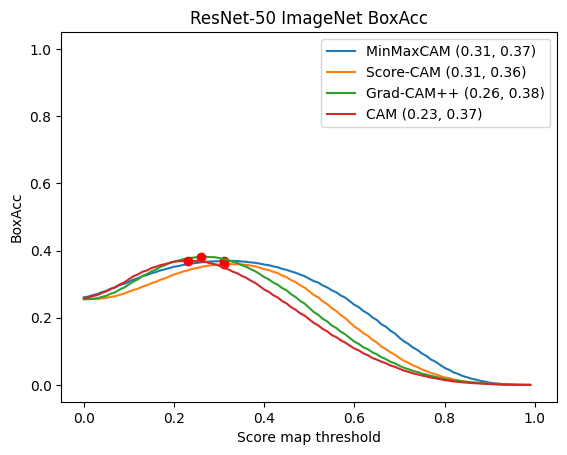
\includegraphics[width=0.7\textwidth]{fig_boxacc_resnet50_imagenet.png}
    \caption[BoxAcc (IoU 50)for ResNet-50 on ImageNet]{Performance at varying operating thresholds. BoxAcc($\tau$) versus score map threshold $\tau$ at IoU threshold 50 for ResNet-50 on ImageNet.}
    \caption*{Source: Author}
    \label{fig:boxacc_resnet50_imagenet}
    \end{center}
\end{figure}

\section{Classification versus localization accuracy}
When comparing classification accuracy with localization accuracy (MaxBoxAccV3 recall) during training, we observed that there is a correlation between both metrics. Fig. \ref{fig:loc_vs_acc_vgg16_gap_cam_synthetic} illustrates that classification accuracy and CAM localization accuracy (MaxBoxAccV3 recall) for VGG16-GAP on each of the validation synthetic datasets, improve during the early epochs of training, until both metrics start converging.

A question is then which checkpoint during training is suitable for localization evaluation? Choe \textit{et al.} \cite{choe2020evaluating} argue that in many cases, the best localization performances are achieved before convergence, that at early epochs, the localization can fluctuate a lot and thus, peak performance is noise rather than real performance. Fig. \ref{fig:loc_vs_acc_resnet50_cam_d1b} illustrates such case for the CAM localization method on ResNet-50 for the d1b synthetic dataset. We clearly see that the maximum value for MaxBoxAccV3 is reached during the early training epochs, and drops around epoch 10 before converging.

To avoid measuring noise, we use an early stop criterion that ends model training when classification accuracy has not improved the best accuracy for five consecutive training epochs. We then take as localization accuracy the value computed at the last epoch on the validation dataset.

\begin{figure}[ht]
\begin{center}
    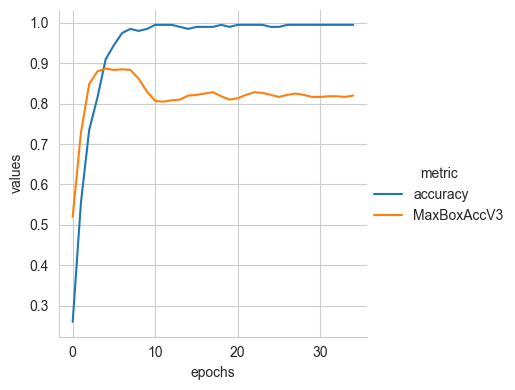
\includegraphics[width=0.6\textwidth]{images/fig_loc_vs_acc_resnet50_cam_d1b.png}
    \caption[Classification versus CAM localization accuracy on ResNet-50 for d1b dataset]{Classification versus CAM localization accuracy on ResNet-50 for d1b dataset.}
    \caption*{Source: Author}
    \label{fig:loc_vs_acc_resnet50_cam_d1b}
\end{center}
\end{figure}

\section{Iterative localization} \label{dis:iterative_localizaiton}
The results of the iterative localization experiments in section \ref{sec:exp_loc_improvements} show that localization recall can be improved using the iterative approach on all localization metrics. Depending on the mask strategy, merge strategy and chosen stop criterion, recall can be improved substantially. In most cases, recall improvement comes at the cost of precision loss when compared with the baseline.

The two parameters that are most important for improving recall, are the merge strategy and the iteration stop criterion. This is understandable as these two parameters directly determine whether predicted bounding boxes will be added to the list of bounding boxes predicted during previous iterations. 

For the synthetic datasets with multiple object instances and in the ImageNet dataset, the experiments using the 'add' merge strategy and iteration stop threshold 1.0 show the most substantial gain in recall but at a large impact on precision. It is easy to see that in this scenario, each iteration can add more bounding boxes, potentially increases matches or mismatches between predicted and ground truth bounding boxes, hence increasing recall in the former and decreasing precision in the latter case.

The experiments with the large and diverse ImageNet dataset shows that there is quite some room for improving localization recall. However, the current iterative approach stills suffers from substantial loss in precision. Precision for the iterative approach is bad because of the bias in ImageNet to images with single object instance. We expect the results to be more in line with other experiments for synthetic dataset if the iterative localization would be done on the ImageNet dataset split by object instance count. We see this as future work.

In our current iterative localization approach, we use bounding boxes predicted in previous iterations as image masks to predict new boxes. As future work it would be interesting to evaluate using the more fine-grained score map as an image mask for improving precision.

\subsection{IoU threshold for merge strategy}
The merge strategy 'drop' or 'unify' is applied only if newly found bounding boxes sufficiently overlap with bounding boxes found during previous iterations. We use a merge threshold parameter to determine whether bounding boxes overlap sufficiently. For our iterative localization experiments, the parameter value was fixed to 20\%. This may not be the optimal value for each merge strategy. To assess the impact of this parameter on localization results, we have run the experiment from section \ref{sec:exp_iter_resnet50_syn} for the CAM method only, using different values for the IoU threshold parameter. The results are illustrated in Fig. \ref{fig:prec_iter_resnet50_syn_iou_d1b}, Fig. \ref{fig:prec_iter_resnet50_syn_iou_d2b}, Fig. \ref{fig:prec_iter_resnet50_syn_iou_d3b} and Fig. \ref{fig:prec_iter_resnet50_syn_iou_d4b} for the respective synthetic datasets d1b, d2b, d3b and d4b. We observe that the higher the IoU threshold is, the more precision and recall for the 'drop' and 'unify' strategy, moves towards the 'add' strategy, i.e., recall becomes better at the cost of precision. Intuitively, the higher the overlap threshold, the more the 'drop' strategy and the 'unify' strategy will behave as the 'add' strategy, because there's a higher probability that bounding boxes will not overlap. In the latter case, the 'stop' and 'unify' strategy will default to the 'add' strategy, as we defined in chapter \ref{ch:methodology}.

\begin{figure}[h]
    \begin{center}       
    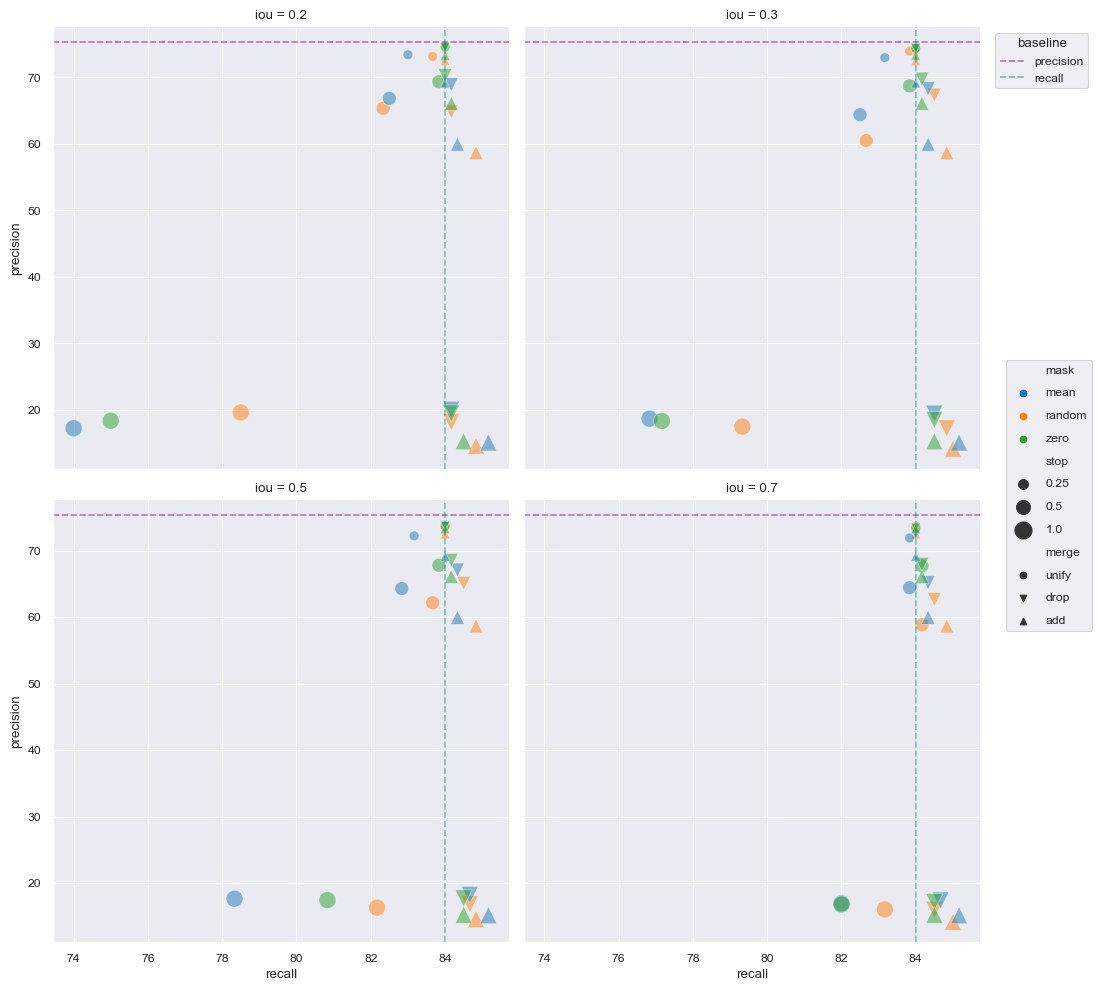
\includegraphics[width=0.99\textwidth]{fig_iter_resnet50_syn_iou_d1b.png}
    \caption[Iterative localization by IoU threshold for ResNet-50 on synthetic dataset d1b]{Iterative localization by IoU threshold for ResNet-50 on synthetic dataset d1b. The cross-hair lines mark the best precision and recall for non-iterative localization.}
    \caption*{Source: Author}
    \label{fig:prec_iter_resnet50_syn_iou_d1b}
    \end{center}
\end{figure}

\begin{figure}[h]
    \begin{center}       
    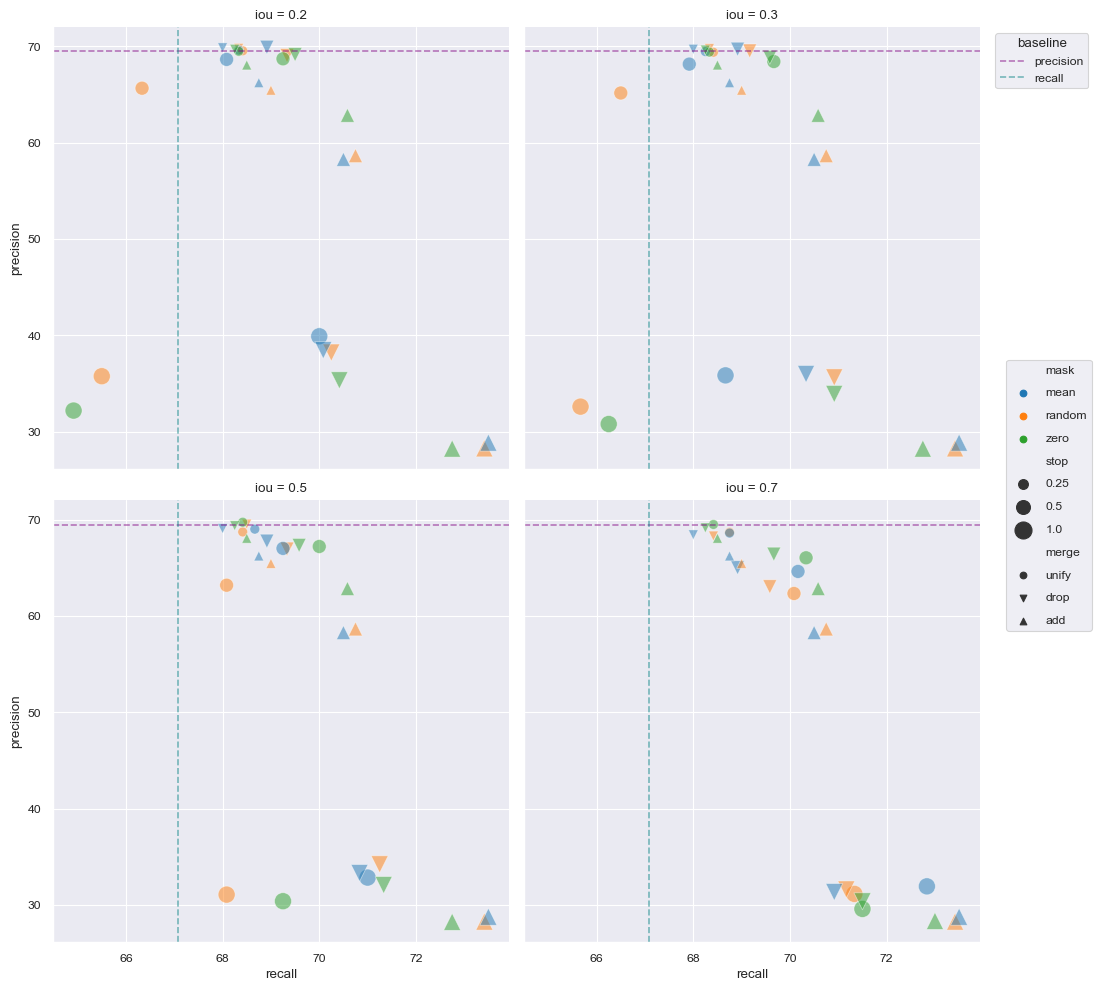
\includegraphics[width=0.99\textwidth]{fig_iter_resnet50_syn_iou_d2b.png}
    \caption[Iterative localization by IoU threshold for ResNet-50 on synthetic dataset d2b]{Iterative localization by IoU threshold for ResNet-50 on synthetic dataset d2b. The cross-hair lines mark the best precision and recall for non-iterative localization.}
    \caption*{Source: Author}
    \label{fig:prec_iter_resnet50_syn_iou_d2b}
    \end{center}
\end{figure}

\begin{figure}[h]
    \begin{center}       
    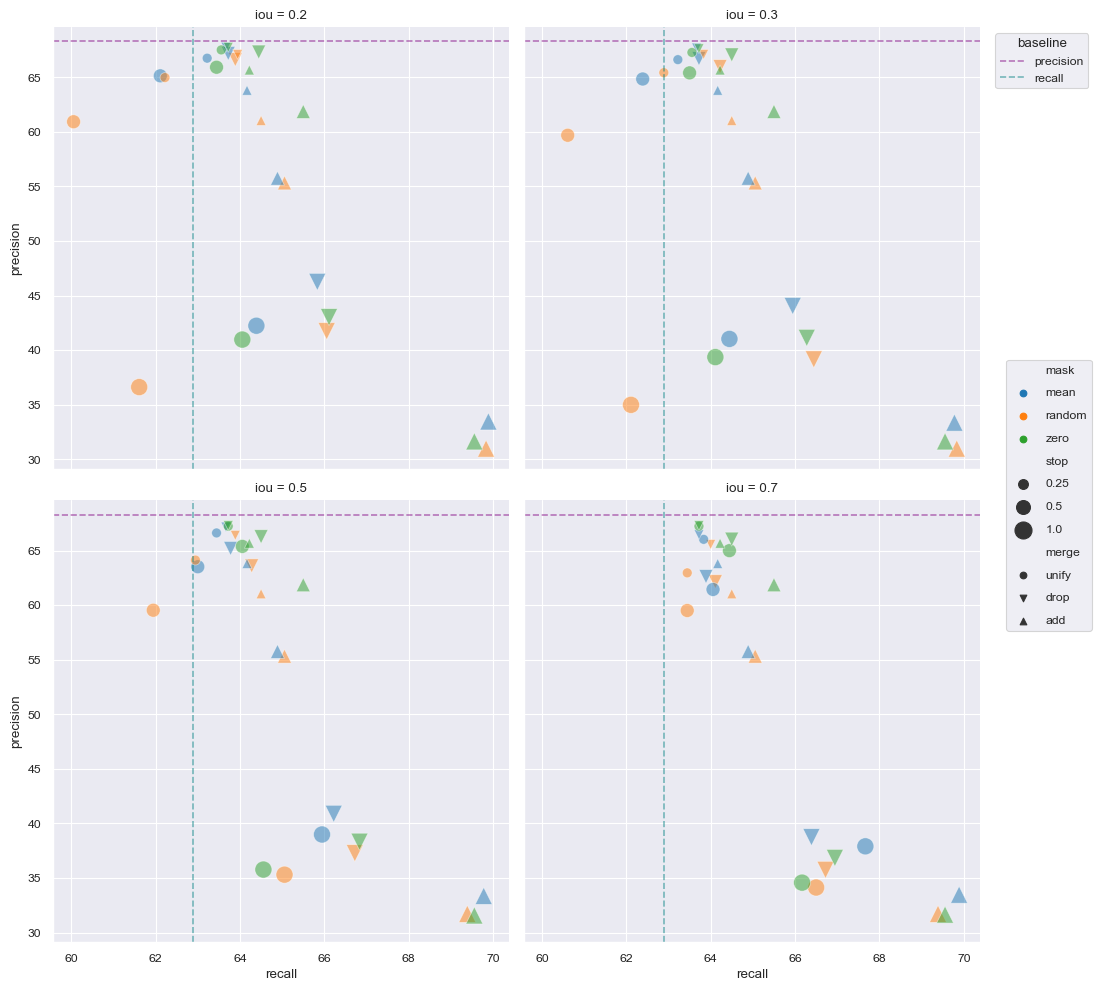
\includegraphics[width=0.99\textwidth]{fig_iter_resnet50_syn_iou_d3b.png}
    \caption[Iterative localization by IoU threshold for ResNet-50 on synthetic dataset d3b]{Iterative localization by IoU threshold for ResNet-50 on synthetic dataset d3b. The cross-hair lines mark the best precision and recall for non-iterative localization.}
    \caption*{Source: Author}
    \label{fig:prec_iter_resnet50_syn_iou_d3b}
    \end{center}
\end{figure}

\begin{figure}[h]
    \begin{center}       
    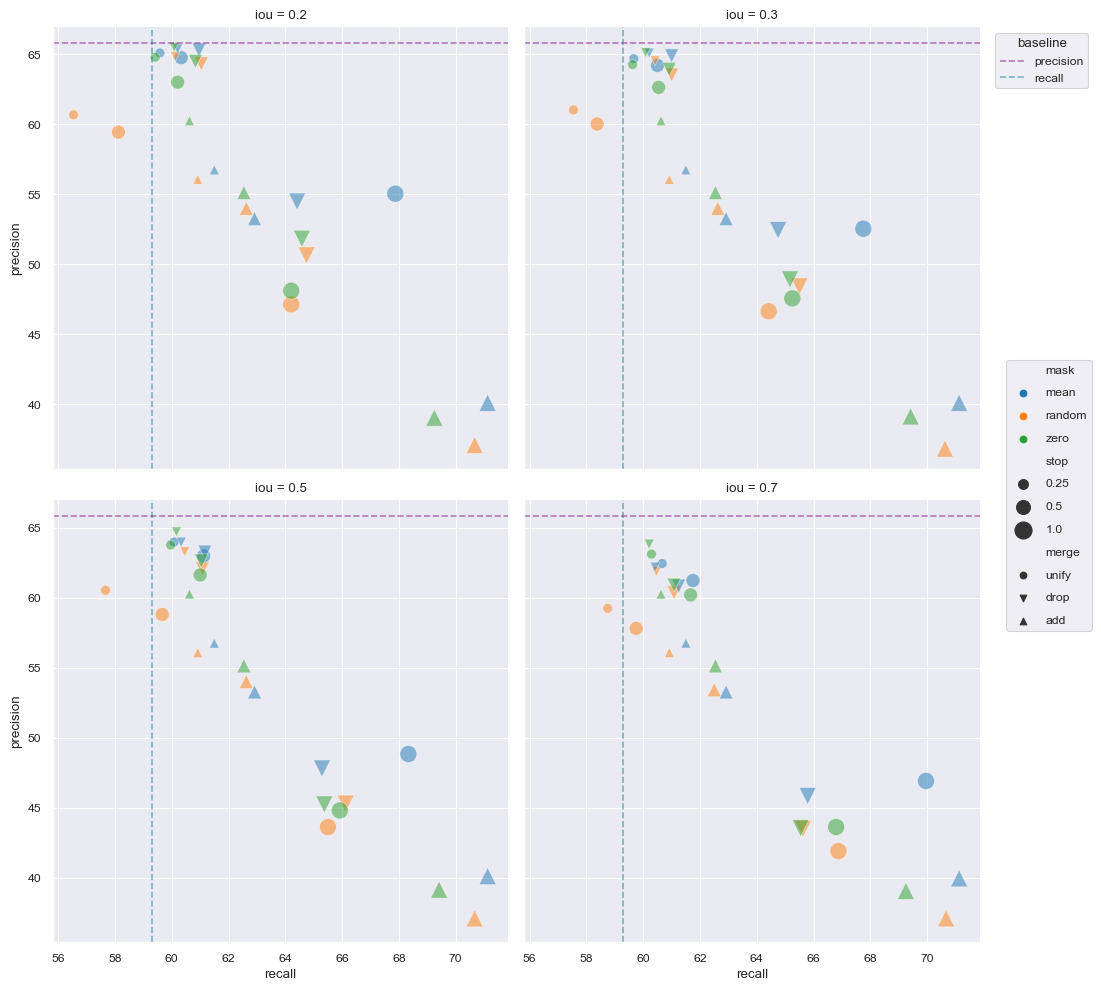
\includegraphics[width=0.99\textwidth]{fig_iter_resnet50_syn_iou_d4b.png}
    \caption[Iterative localization by IoU threshold for ResNet-50 on synthetic dataset d4b]{Iterative localization by IoU threshold for ResNet-50 on synthetic dataset d4b. The cross-hair lines mark the best precision and recall for non-iterative localization.}
    \caption*{Source: Author}
    \label{fig:prec_iter_resnet50_syn_iou_d4b}
    \end{center}
\end{figure}

\chapter{Conclusion}

% feedback Benjamin

-	Afronden \\
-	Kort het verhaal uitleggen \\
-	In this thesis we instroduced a new method to evaluate multi-instance wsol \\
-	This are our conclusions... \\
-	Bestaande methodes niet voldoende maar onze methode doet het beter in die en die opzichten. \\

\clearpage\nocite{*}
\bibliographystyle{unsrt}
\phantomsection
\addcontentsline{toc}{chapter}{Bibliography}
\bibliography{chapters/bibliography} 

\end{document}
